\def\thudbabelopt{english}
\PassOptionsToPackage{usenames}{xcolor}
\PassOptionsToPackage{dvipsnames}{xcolor}
\PassOptionsToPackage{table}{xcolor}
\documentclass[target=bach,aauheader=]{thud}

%% --- Information about the thesis --- %%
\course{Internet of Things, Big Data and Web}
\title{Comparison of tools for the formal verification of MTProto 2.0}
\author{Alessandro Zanatta}
\supervisor{Prof.\ Marino Miculan}
\cosupervisor{Prof.\ Nicola Vitacolonna} % TODO: Is Vitacolonna considered a supervisor?
%% Other available fields: \reviewer, \tutor, \chair, \date (anno accademico, calcolato in automatico), \rights

%% --- Suggested packages ---
%% pdfx: per generare il PDF/A per l'archiviazione. Necessario solo per la versione finale
\usepackage[a-1b]{pdfx}
%% hyperref: Regola le impostazioni della creazione del PDF... più tante altre cose. Ricordarsi di usare l'opzione pdfa.
\usepackage[pdfa]{hyperref}
%% tocbibind: Inserisce nell'indice anche la lista delle figure, la bibliografia, ecc.

%% --- Stili di pagina disponibili (comando \pagestyle) ---
%% sfbig (predefinito): Apertura delle parti e dei capitoli col numero grande; titoli delle parti e dei capitoli e intestazioni di pagina in sans serif.
%% big: Come "sfbig", solo serif.
%% plain: Apertura delle parti e dei capitoli tradizionali di LaTeX; intestazioni di pagina come "big".

%% --- Other packages --- %%ì
\usepackage{msc} % Protocol graphical representation
\usepackage{mathtools}
\usepackage{amssymb}
\usepackage{enumitem}
\usepackage[justification=centering]{caption} % Used to have always centered captions
\usepackage{cleveref} % better references
\usepackage{graphicx} % for images
\usepackage{textgreek} % greek letters out of math mode
\usepackage{caption} % captions for equations (outside of floats, in general)
\usepackage{listings}
\usepackage[super]{nth}
\usepackage{multicol}
\usepackage[T1]{fontenc}
\usepackage{courier} % Font for listings
\usepackage{subfig}
\usepackage{multirow}

\setlist[description]{style=nextline}

\newcommand\keywordstyle[1]{{\scriptsize\color{MidnightBlue}\bfseries\mathversion{bold}#1}}

\lstset{
  numbers=left,
  xleftmargin=\parindent,
  basicstyle=\footnotesize\linespread{1}\ttfamily,
  breaklines=true,
  captionpos=b,
  aboveskip=10pt,
  belowskip=10pt
}
\graphicspath{ {./images/}, {./plots/} } % images path

\DeclareCaptionType{equ}[][]

%% --- Commands --- %%
\newcommand\setmscoptions{
  % \setlength{\levelheight}{1.5 \levelheight}%
  % \setlength{\instwidth}{3cm}
  \setmsckeyword{}
  \drawframe{no}
  \centering
}


% Multiline comments
\newcommand{\comment}[1]{}

\newcommand*{\Z}{\mathbb{Z}}
\newcommand*{\Q}{\mathbb{Q}}

%% Taken from https://hal.inria.fr/file/index/docid/955869/filename/sapic.tex
\newcommand{\msrewrite}[1]{\mathrel{-\hspace{-2pt}[#1]\hspace{-4pt}\to}}
\newcommand{\emptyrule}{\ensuremath{[]}\xspace}
\newcommand{\msr}[3]{\ensuremath{[#1] \msrewrite{#2} [#3]}}
%% -------------- %%

\newcommand{\msrnolabel}[2]{\ensuremath{[#1] \rightarrow [#2]}}
\newcommand{\msrsetminus}{\ensuremath{\setminus^\#}}
\newcommand{\msrcap}{\ensuremath{\cap^\#}}
\newcommand{\msrcup}{\ensuremath{\cup^\#}}
\newcommand{\msrin}{\ensuremath{\in^\#}}
\newcommand{\msrsubseteq}{\ensuremath{\subseteq^\#}}
\newcommand{\lin}[1]{\ensuremath{lin\left(#1\right)}}
\newcommand{\pers}[1]{\ensuremath{pers\left(#1\right)}}

\newcommand{\fact}[2]{\ensuremath{\mbox{!#1}\left(#2\right)}}
\newcommand*{\myexp}{\hat{\mkern6mu}}

% pi-calculus
\newcommand{\apicpc}[2]{\ensuremath{P\ |\ Q}}
\newcommand{\apicin}[3]{\ensuremath{#1\left(#2\right).#3}}
\newcommand{\apicout}[3]{\ensuremath{\overline{#1}\left<#2\right>.#3}}
\newcommand{\apicrep}[1]{\ensuremath{!#1}}
\newcommand{\apicnew}[2]{\ensuremath{#1.#2}}
\newcommand{\apicif}[3]{\ensuremath{\mbox{if}\ #1\ \mbox{then}\ #2\ \mbox{else}\ #3}}
\newcommand{\apicevent}[2]{\ensuremath{\mbox{event}\ \mbox{#1}\left(#2\right)}}

% MTProto encryption symbols/functions
\newcommand{\func}[2]{\ensuremath{\mbox{#1}\left(#2\right)}}
\newcommand{\enc}[2]{\ensuremath{\left\{#1\right\}_{#2}}}
\newcommand{\sha}[2]{\ensuremath{\func{sha#1}{#2}}}
\newcommand{\kdf}[1]{\ensuremath{\func{kdf}{#1}}}
\newcommand{\fpk}[1]{\ensuremath{\func{fpk}{#1}}}
\newcommand{\hash}[1]{\ensuremath{\func{hash}{#1}}}
\newcommand{\modexp}[3]{\ensuremath{#1^#2 \mod{#3}}}
\newcommand{\key}[1]{\ensuremath{k_{#1}}}
\newcommand{\newkey}[1]{\ensuremath{k'_{#1}}}
\newcommand{\group}[1]{\ensuremath{\Z_{#1}}}
\newcommand{\attack}[1]{\ensuremath{\func{attacker}{#1}}}

% spacing in math multiline mode
\setlength{\jot}{1pt}

% Commands for spelling consistency 
\newcommand{\pic}{\textpi-calculus}
\newcommand{\apic}{applied \textpi-calculus}
\newcommand{\Apic}{Applied \textpi-calculus}

\newcommand{\Hornc}{Horn clause}
\newcommand{\Horncs}{Horn clauses}

\newcommand{\pfs}{perfect forward secrecy}
\newcommand{\Pfs}{Perfect forward secrecy}
\newcommand{\PFS}{Perfect Forward Secrecy}

\newcommand{\cchat}{cloud chat}
\newcommand{\Cchat}{Cloud chat}
\newcommand{\cchats}{cloud chats}
\newcommand{\Cchats}{Cloud chats}

\newcommand{\schat}{secret chat}
\newcommand{\Schat}{Secret chat}
\newcommand{\schats}{secret chats}
\newcommand{\Schats}{Secret chats}

\newcommand{\Uks}{Unknown key-share}
\newcommand{\uks}{unknown key-share}

\newcommand{\mitm}{man-in-the-middle}
\newcommand{\MitM}{Man-in-the-Middle}
\newcommand{\DiHe}{Diffie-Hellman}

\newcommand{\MMNV}{M. Miculan and N. Vitacolonna}
\newcommand{\SBWAM}{S. Blake-Wilson and A. Menezes}
\newcommand{\BLANC}{B. Blanchet}

\newcommand{\Mrss}{Maximum resident set size}
\newcommand{\mrss}{maximum resident set size}
\newcommand{\MRSS}{Maximum Resident Set Size}

\newcommand{\WCT}{Wall Clock Time}
\newcommand{\Wct}{Wall clock time}
\newcommand{\wct}{wall clock time}

%% -------------------------------------------------------------------------------- %%
%% Languages listings                                                               %%
%% -------------------------------------------------------------------------------- %%
\lstdefinelanguage{tamarin}
{
  keywordstyle=\color{MidnightBlue}\bfseries,
  keywordstyle=[2]\itshape,
  keywordstyle=[3]\color{Green}\bfseries,
  keywordstyle=[4]\color{RedViolet}\bfseries,
  alsoletter={^,==>,|,&,.,-},
  keywords={Out, In, K, KU, Fr, ^, senc, sdec, adec, aenc, ~, All, Ex, not, ., &, |, ==>, diff, pk, h},
  keywords=[2]{},
  keywords=[3]{},
  keywords=[4]{sources, exists-trace, rule, lemma, restriction, let, in, theory, builtins, begin, end, hashing},
  sensitive=true,
  morecomment=[l][\color{OliveGreen}\itshape]{//},
  morecomment=[n][\color{OliveGreen}\itshape]{/*}{*/},
  morestring=[b]',
  stringstyle=\color{BrickRed},
  literate=%
  {∃}{{\keywordstyle{$\exists$}}}1
  {∀}{{\keywordstyle{$\forall$}}}1
  {∧}{{\keywordstyle{$\land$}}}1
  {∨}{{\keywordstyle{$\lor$}}}1
  {¬}{{\keywordstyle{$\neg$}}}1
  {==>}{{\keywordstyle{ $\Longrightarrow$}}}2
}

\lstdefinelanguage{proverif}
{
  keywordstyle=\color{MidnightBlue}\bfseries,
  keywordstyle=[2]\itshape,
  keywordstyle=[3]\color{Orange}\bfseries,
  keywordstyle=[4]\color{RedViolet}\bfseries,
  keywords={|, !, bitstring},
  keywords=[2]{},
  keywords=[3]{false, true},
  keywords=[4]{type, channel, fun, reduc, let, table, query, insert, phase, get, out, event, in, ., ;, attacker, forall, if, else, new, then, typeConverter, process},
  sensitive=true,
  morecomment=[n][\color{OliveGreen}\itshape]{(*}{*)},
  morestring=[b]",
  morekeywords={.}
}

%% -------------------------------------------------------------------------------- %%
%% Document start                                                                   %%
%% -------------------------------------------------------------------------------- %%
\begin{document}
\maketitle

%% Dedica (opzionale)
% \begin{dedication}
%   Al mio cane,\par per avermi ascoltato mentre ripassavo le lezioni.
% \end{dedication}

%% Ringraziamenti (opzionali)
\acknowledgements
Ringraziamenti vari qua

%% Sommario (opzionale)
% \abstract
% Un bell'abstract va qua!

%% Indice
\tableofcontents

%% Lista delle tabelle (se presenti)
%\listoftables

%% Lista delle figure (se presenti)
%\listoffigures

%% Corpo principale del documento
\mainmatter

%% Capitolo
\chapter{Introduction}
\label{section:introduction}

Security protocols are used every day by billions of users and applications to guarantee a certain degree of security and privacy over communications happening on the (insecure) Internet (SSH \cite{rfc4251} and TLSv1.3 \cite{TLSv1.3_specs} protocols are just a few famous examples). Although, there is a catch: designing such protocols has been proven to be very error-prone. As an example, consider the Needham-Schroeder public-key protocol \cite{NSPK}, which has been believed to be secure for almost 20 years - before a fatal flaw was found and corrected \cite{NSPK_LoweGavin}.

Given the importance of the correctness of such protocols and the difficulties for designers to ensure it, it has been necessary to \textit{formally} prove the absence of security vulnerabilities. Towards this aim, a set of tools has been developed to assist the designing of a new protocol.

In this thesis, we are going to compare two tools: Tamarin prover and Proverif. In particular, we will compare them for the formal verification of Telegram's protocol: MTProto2.0. The protocol has already been analyzed and formalized with Proverif by \MMNV{} \cite{MTProto2-Proverif-impl}, and it has been discussed in the associated paper \cite{MTProto2-Proverif}. The formalization in Tamarin will be based on this work, with remarkable differences due to the diverse nature of the two tools.


\chapter{Symbolic and computational model}
First of all, let us consider the different types of approaches to security protocol analysis. The two categories of techniques are shown in \cref{fig:symbolic-computational-model}. We will proceed to examine them in this chapter.

\begin{figure}[t]
    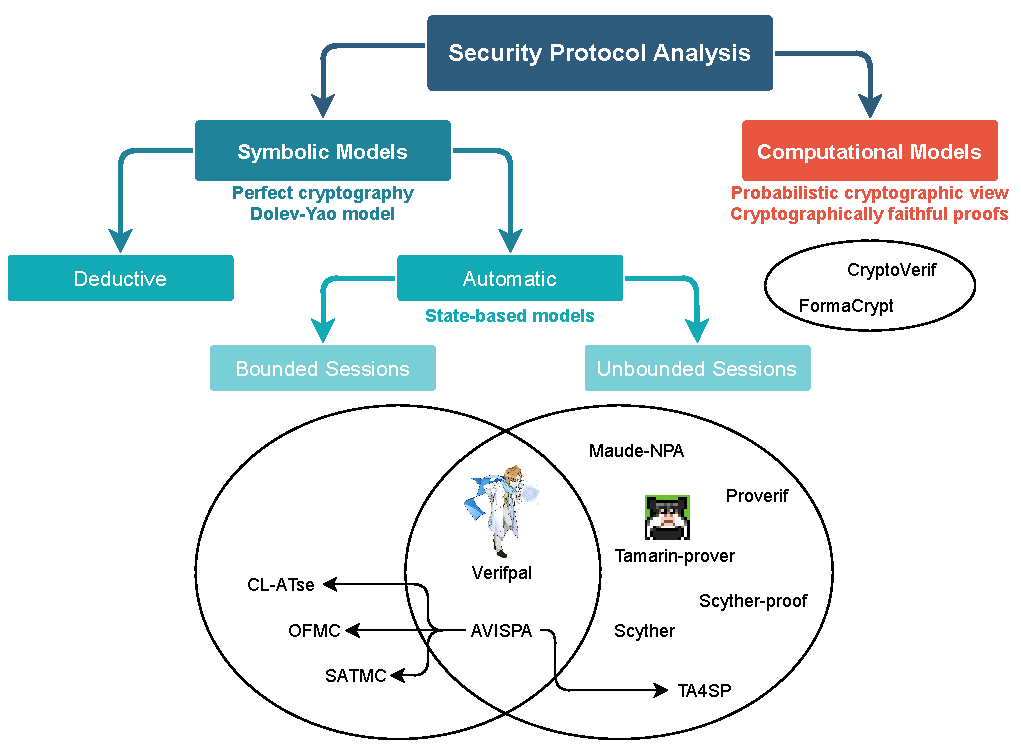
\includegraphics[scale=0.9]{symbolic-computational-model}
    \centering
    \caption{Symbolic and computational models and available tools.\\Inspired by a representation from Nicola Vitacolonna.}
    \label{fig:symbolic-computational-model}
\end{figure}

In the \textit{symbolic model} (often called Dolev-Yao model) \cite{Dolev-Yao}, the cryptographic primitives are considered as black-box and are represented using function symbols, the messages are terms and the adversary can only use defined primitives. An important aspect to note of this model is that it assumes \textbf{perfect cryptography}. As an example, consider the case in which there are two function symbols (\textbf{enc} and \textbf{dec}, used to encrypt and decrypt), a message \textit{m} and a key \textit{k} and the following equality is defined:

\begin{equation}
    \mbox{dec}\left(\mbox{enc}\left(m, k\right), k\right) = m
\end{equation}

Following from the equation $-$ and considering the perfect cryptography assumption $-$ it is possible to decrypt $\mbox{enc}\left(m, k\right)$ if and only if \textit{k} is known \cite{SymbolicComputationalBlanchet}.

In the \textit{computational model} the messages are bitstrings, the cryptographic primitives are functions from bitstrings to bitstrings, the attacker is modeled as a probabilistic Turing machine.
A security property in this model is considered to hold when the probability that it does \textit{not} hold is negligible. For instance, the previously discussed shared-key encryption can be modeled using the same equation. However, the security of encryption is expressed by stating that the attacker has an insignificant probability of breaking the primitive (e.g. decrypting the message without having the key). Security proofs using this model are usually stronger, but this comes to the cost of long, difficult, tedious, highly error-prone proofs (as stated by INRIA researchers \cite{ComputationalAnalysisCryptoSystemsINRIA}). Finally, as pointed to by Blanchet \cite{SymbolicComputationalBlanchet}, the computational model is indeed just a \textit{model} and ignores many aspects of reality and potential attacks, e.g. faulty attacks like the one affecting processors computing RSA signatures \cite{RSAFaultAttack}.

Of all the tools in \cref{fig:symbolic-computational-model}, we are going to discuss two automatic tools that employ a symbolic model: \href{https://prosecco.gforge.inria.fr/personal/bblanche/proverif/}{Proverif} and \href{https://tamarin-prover.github.io/}{Tamarin prover}. We will also refer to Tamarin prover as Tamarin for brevity.

We choose to focus on the tools that exploit the symbolic model as it makes it possible to automate proofs. Notice that termination is still not always guaranteed\footnote{It depends on the tool. Both Proverif and Tamarin may not terminate. Proverif proofs may end with an inconclusive result, while Tamarin will always give the correct answer (assuming termination). Other tools, like Scyther \cite{Scyther}, always terminate by limiting the growth of some parameters. More details about this problem will be discussed in \cref{sec:difficulties-analysis-symbolic}.}. From now on we will always refer to the symbolic model implicitly.

\section{Difficulties in the security protocol analysis in the symbolic model}
\label{sec:difficulties-analysis-symbolic}
Two main problems affect most automatic tools for security protocol analysis: \textbf{infinite state space} and \textbf{undecidability}.

At a high level, to verify a protocol in the symbolic model, one computes the set of terms that the adversary knows. If a certain term does not belong to this set, then the term is considered secret \cite{SymbolicVerificationBlanchet}. The difficulty is that the set of terms is infinite. Specifically, we have to deal with three sources of infinity when analyzing a protocol:
\begin{description}
    \item[\textbf{Messages}] - the adversary can produce messages of any arbitrary size;
    \item[\textbf{Sessions}] - as many attacks are possible only when multiple sessions are executed in parallel, symbolic models often use an unbounded number of sessions;
    \item[\textbf{Nonces}] - if we have an unbounded number of session, then we also must have an unbounded number of nonces to use in those sessions.
\end{description}

There have been various ways of tackling this problem:
\begin{itemize}
    \item{It is possible to decide to bound every source of infinity. In this case, the state space is finite. This method was used, for example, by Lowe \cite{LoweNeedhamSchroederPK} and SATMC \cite{SATMC};}

    \item{We can bound the number of executions of the protocol. This still leads to an infinite state space, but \cite{SymbolicModelNPCompleteInsecurity} have shown that insecurity is NP-complete;}

    \item{If we do not force any bound, the problem becomes undecidable \cite{SymbolicModelUndecidability1} \cite{SymbolicModelUndecidability2}. As pointed out by \cite{SymbolicVerificationBlanchet}, no automatic tool that always terminates and solves the problem can exist. In general, it is not possible to determine if a certain proof will, eventually, end. \Cref{fig:undecidability} shows the boundary of decidability. As evidenced by the diagram, the problem is decidable if and only if we bound at least two sources of infinity out of three.

                Of course, there are several approaches to confront this problem:

                \begin{itemize}
                    \item{Rely on help from the user. This is the approach chosen by Tamarin \cite{TamarinFoundations}, which allows for semi-automatic proofs. In Tamarin, possible resolution steps are ranked by the system, but the user can choose which to solve first;}
                    \item{Another possibility is to have tools that may return an inconclusive result $-$ yet are supposed to work correctly in most cases. Proverif follows this approach \cite{SymbolicVerificationBlanchet};}
                    \item{The last approach is to allow non-termination.}
                \end{itemize}
          }
\end{itemize}


\begin{figure}[t]
    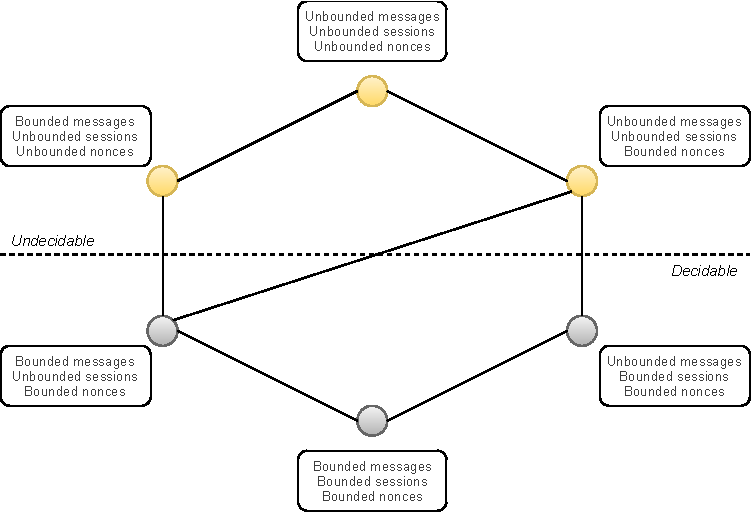
\includegraphics{undecidability}
    \centering
    \caption{Decidability of termination.\\Inspired by a representation from Nicola Vitacolonna.}
    \label{fig:undecidability}
\end{figure}

\chapter{Tools foundations}
In this section, we will look at the foundations of the analyzed tools, Proverif and Tamarin prover.


\section{Proverif}
Let us start with a brief overview of Proverif internal reasoning. For more information, please refer to \cite{SymbolicComputationalBlanchet, SymbolicVerificationBlanchet, ProverifManual}.

\subsection{High level view}
Proverif protocols and security properties are based on an extended version of the \pic{} (the \textit{applied} \pic{}). The tool also allows the user to define constructors, destructors and equations\footnote{Destructors are basically used to de-construct some previously constructed term (e.g. decryption of an encrypted ciphertext), while equations represent term equality of some sort (e.g. commutativity of multiplication).}, which form the cryptographic primitives. The protocol is then automatically translated to a set of \Horncs{}. Using this abstract representation of the protocol (based on \Horncs{}), the Proverif verifier uses a resolution algorithm on such clauses that allow for verification of security properties \cite{SymbolicComputationalBlanchet}.
A graphical representation of the whole process is given in \cref{fig:proverif-verification-method}.

It is important to note that Proverif is not complete. This means that it may find false attacks. Moreover, it may not terminate, but it has been proven to be precise and efficient enough in practice by many case studies (the following is a non-exhaustive list of examples \cite{10.1145/1266977.1266978, ABADI20053, hal-01575923, MTProto2-Proverif}).

We will now proceed with an overview of \pic{} and \Horncs{}.

\begin{figure}[t]
    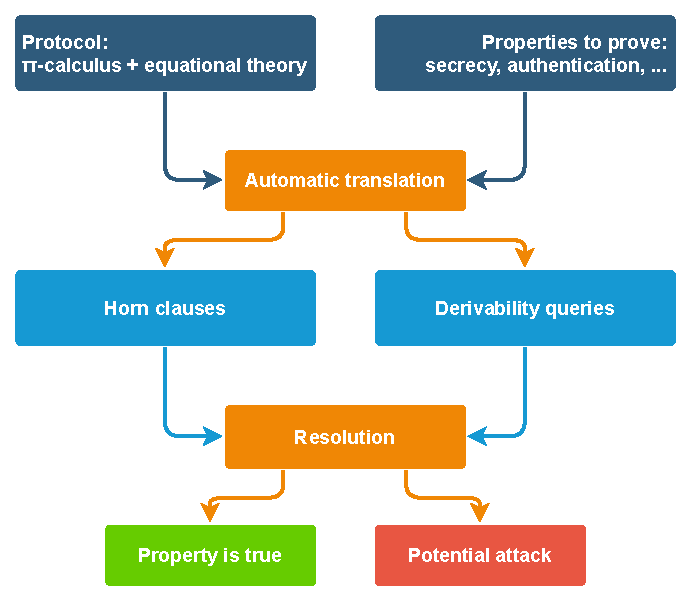
\includegraphics{proverif-verification-method}
    \centering
    \caption{Proverif verification method.\\Inspired by a representation from \BLANC{} \cite{SymbolicComputationalBlanchet}.}
    \label{fig:proverif-verification-method}
\end{figure}

\subsection{\pic{} and \apic{}}
\label{subsec:pic-apic}

The \pic{} \cite{pi-calculus-book} is a (minimal) programming language that models a system communicating on channels. It belongs to the \textit{process calculi} family, which is generally used to model concurrent systems. As Proverif uses the \textit{applied} \pic{} (which is an extension of standard \pic{}{}), we will briefly present its syntax in the rest of this section.

The following description of \apic{} references articles \cite{applied-pi-calculus-private-auth, applied-pi-calculus-abadi-1, applied-pi-calculus-abadi-2}. Please refer to these resources for further information and a more formal or in-depth description. For brevity, we only define the main features of \apic{} in \cref{subsub:syntax-apic}.

\paragraph{Overview of the syntax of the \apic{}}
\label{subsub:syntax-apic}

A \textit{signature \textSigma} is composed by a finite number of functions symbols, each with its own integer arity. Given such signature, together with an infinite set of names and an infinite set of variables, the set of \textbf{terms} is defined by the grammar:

\begin{equation}
    \label{eq:apic-terms}
    \begin{aligned}
        U, V & ::=                        \\
             & a, b, \ldots               \\
             & x, y, \ldots               \\
             & \func{f}{U_1, \ldots, U_l}
    \end{aligned}
    \qquad
    \begin{aligned}
        \mbox{term} & \mbox{s}                       \\
                    & \mbox{name}                    \\
                    & \mbox{variable}                \\
                    & \mbox{constructor application}
    \end{aligned}
\end{equation}

where $f \in \Sigma$ and $l$ matches the arity of $f$. Next, we define a grammar for processes, which is shown in \cref{eq:apic-processes}. As pointed to by Microsoft researchers, this grammar is very similar to the \pic{} \cite{applied-pi-calculus-private-auth}. We will omit to define differences from standard \pic{} as we have not formally defined \pic{} either.

\begin{equation}
    \label{eq:apic-processes}
    \begin{aligned}
        P, Q & ::=                 \\
             & 0                   \\
             & \apicout{N}{M}{P}   \\
             & \apicin{N}{x}{T}{P} \\
             & \apicpc{P}{Q}       \\
             & \apicrep{P}         \\
             & \apicnew{a}{T}{P}   \\
             & \apicif{M}{P}{Q}
    \end{aligned}
    \qquad
    \begin{aligned}
        \mbox{proc} & \mbox{esses}                                         \\
                    & \mbox{null process}                                  \\
                    & \mbox{output to channel N of message M}              \\
                    & \mbox{input from channel N of message M with sort T} \\
                    & \mbox{parallel composition}                          \\
                    & \mbox{replication}                                   \\
                    & \mbox{fresh value of sort T}                         \\
                    & \mbox{conditional}
    \end{aligned}
\end{equation}

The null process $0$ does nothing;
$\apicout{N}{M}{P}$ ($\apicin{N}{x}{T}{P}$) outputs (gets) the message M (of sort $x$) into (from) channel N and then continues with process $P$; Notice that getting a message from a channel is a blocking operation;
$\apicpc{P}{Q}$ is the parallel composition of $P$ and $Q$;
The process $\apicrep{P}$ effectively behaves as an infinite number of copies of $P$ running in parallel (\textit{unbounded} replication);
$\apicnew{a}{T}{P}$ creates a new fresh value of sort $T$, before proceeding with process $P$;
$\apicif{M}{P}{Q}$ is a standard conditional.

\comment{
$\apiclet{x}{T}{D}{P}{Q}$ is used to apply destructors or assign some term $D$ to a variable $x$ (of sort $T$);
}

\subsection{\Horncs{}}

As we said earlier, Proverif's analysis is based on \Horncs{}. Let us define them.

The class of Horn formulas is obtained by restricting the form of the conjuncts in a proposition in conjunctive normal form. Consider a proposition $A$ in conjunctive normal form $C_1 \land \ldots \land C_n$, where each $C_i$ is a conjunction of either positive or negative literals. A is a \Hornc{} if and only if each $C_i$ contains at most one positive literal \cite{DOWLING1984267,horn_1951}. Additionally, every variable in a clause is implicitly universally quantified.


\subsection{Intuition for the translation to \Horncs{}}
For this section we will consider \Horncs{} in the following form: $F_1 \land \ldots \land F_n \Rightarrow F$.
Additionally, the literal $\attack{x}$ will be used to denote that the attacker knows the term $x$.

Proverif automatically translates cryptographic primitives, attacker capabilities, and the protocol itself to \Horncs{}. In the following paragraphs, we will show some translations that Proverif applies. Most of the examples are taken from \BLANC{} \cite{blanchet:hal-01110425}.

\paragraph{Representation of cryptographic primitives}
As already seen, Proverif represents cryptographic primitives as constructors and destructors. The constructors are the functions that explicitly appear in the terms that represent messages. A destructors $g$ is defined as a set $\func{def}{g}$ of rewrite rules of the form $g\left(M_1, \ldots, M_n\right) \rightarrow M$, where $M_1, \ldots, M_n, M$ are terms that contain variables and constructors and the variables in $M$ all occur in $M_1, \ldots, M_n$.


\paragraph{Representation of attacker capabilities}
During its computation, the attacker can apply constructors and destructors. Let us define a constructor of arity $n$ as $\func{f}{x_1, \ldots, x_n}$. We can model it with the following clause:

\begin{equation}
    \attack{x_1} \land \ldots \land \attack{x_n} \Rightarrow \attack{\func{f}{x_1,\ldots,x_n}}
\end{equation}

This is consistent with the symbolic model: the adversary needs to know every term to apply a constructor.
Now, suppose that $g$ is a destructor. For each rewrite rule $\func{g}{M_1 \land \ldots \land M_n} \rightarrow M$ in $\func{def}{g}$ we have the following clause:

\begin{equation}
    \attack{M_1} \land \ldots \land \attack{M_n} \Rightarrow \attack{M}
\end{equation}

Notice that the destructor did not appear in the \Hornc{}, and never will. Instead, we use pattern matching to model them. For example, let us show how we can model public-key encryption:

\begin{equation}
    \begin{alignedat}{3}
        & \mbox{aenc} \qquad && \attack{m} \land \attack{pk} \Rightarrow \attack{\func{aenc}{m, pk}}            \\
        & \mbox{pk} \qquad   && \attack{sk} \Rightarrow \attack{\func{pk}{sk}}                                  \\
        & \mbox{adec} \qquad && \attack{\func{aenc}{m, \func{pk}{sk}}} \land \attack{sk} \Rightarrow \attack{m}
    \end{alignedat}
\end{equation}

The first two equation model the constructors $\func{aenc}{m, pk}$ and $\func{pk}{sk}$. The third models asymmetric decryption, defined as $\func{adec}{\func{aenc}{m, \func{pk}{sk}}, sk}$.

\sloppy We also model a revealing signing scheme, formed by two constructors $\func{sign}{m, sk}$ and $\func{pk}{sk}$ and from the rewrite rules $\func{getmess}{\func{sign}{m, sk}} \rightarrow m$ and $\func{verify}{\func{sign}{m, sk}, \func{pk}{sk}} \rightarrow m$, respectively used for message revealing and for signature verification. \Cref{eq:signing-horn-clauses} shows the representation of this primitives as \Horncs{}.

\begin{equation}
    \label{eq:signing-horn-clauses}
    \begin{alignedat}{3}
        & \mbox{sign} \qquad    && \attack{m} \land \attack{sk} \Rightarrow \attack{\func{sign}{m, sk}}            \\
        & \mbox{getmess} \qquad && \attack{\func{sign}{m, sk}} \Rightarrow \attack{m}                              \\
        & \mbox{verify} \qquad  && \attack{\func{sign}{m, sk}} \land \attack{\func{pk}{sk}} \Rightarrow \attack{m}
    \end{alignedat}
\end{equation}

\paragraph{Representation of the protocol}

Let us show how the protocol below can be written as \Horncs{}. We additionally leave to the attacker the task of starting the protocol, that is, the attacker will send the public key of the responder to A.

\begin{enumerate}
    \label{enum:protocol}
    \item A $\rightarrow$ B: $\func{aenc}{\func{sign}{k, skA}, pkB}$
    \item B $\rightarrow$ A: $\func{senc}{m, k}$
\end{enumerate}

The responder of the protocol can either be B or the attacker. In both cases, we can model this with:

\begin{equation}
    \attack{\func{pk}{x}} \Rightarrow \attack{\func{aenc}{\func{sign}{k, skA}, \func{pk}{x}}}
\end{equation}

When B receives the message, he decrypts it with his secret key $skB$. Then, B tests the signature evaluating $\func{verify}{x', pkA}$, which succeeds if and only if $x' = \func{sign}{y, skA}$. If so, B sends a secret constant $m$ using the encryption key $k$. We assume that the attacker relays the message coming from A, and intercepts the message sent by B. Hence, the following clause models the second message of the protocol:

\begin{equation}
    \attack{\func{enc}{\func{sign}{y, skA}, \func{pk}{skB}}} \Rightarrow \attack{\func{senc}{m, y}}
\end{equation}






\section{Tamarin prover}
\label{sec:tamarin-foundations}
In this section, we will see an overview of Tamarin's foundations and internal reasoning.
For a more in-depth description and further information, see the Tamarin foundations paper \cite{TamarinFoundations} or the extended foundations paper \cite{TamarinFoundationsExtended}.

\subsection{High level view}
First of all, let us examine a high-level picture of Tamarin.

The security property model of Tamarin is based on labeled multiset rewriting rules to specify protocols and adversary capabilities, a guarded fragment\footnote{Only a few examples of formulas respecting the guarded fragment of first-order logic used by Tamarin will be given in \cref{sub:guarded-formulas}. See \cite{FragmentFirstOrderLogicPaper} for a rigorous definition from a mathematical point of view.} of first-order logic to specify security properties\footnote{Security properties in Tamarin will also be referred to as \textit{lemmas}.} and functions and equational theories to model the algebraic properties of cryptographic protocols \cite{TamarinFoundations}.

Tamarin uses a novel constraint-solving algorithm to validate or falsify lemmas.

In other words, Tamarin allows to specify a labeled transition system that induces a set of traces and offers automatic verification of such traces using a guarded fragment of first-order logic to specify ``good" traces. Tamarin then tries to prove the negation of the specified ``good" traces.

Tamarin also offers built-in equational theories \cite{TamarinProverManual}. A brief overview will be given in \cref{sub:built-in-equational-theories}.

\subsection{Terminology}
\label{subsec:tamarin-foundations-terminology}
As reported earlier, multiset rewriting rules are used to specify adversary capabilities and protocols. More precisely, a \textit{set} of \textit{labelled} multiset rewriting rules are used.

The ingredients of this multiset rewriting system are the following:

\begin{description}[style=nextline]
    \item[Terms] which can be essentially thought of as messages. Terms can be of three different sorts. The more general sort is the \textit{msg} sort, which has two incomparable sub-sorts \textit{fresh} and \textit{pub} for fresh and public names, respectively;
    \item[Facts] which model information in the protocol. Facts have an arity, can be linear or persistent and are composed by terms. Linear facts model resources that can be consumed once, while persistent facts can be consumed an arbitrary number of times (and are prefixed by an exclamation mark). By convention, facts always start with a capital letter;
    \item[Special facts] Four facts are reserved and are used to model the freshness of a message $t$ ($\mbox{\textbf{Fr}}\left(t\right)$), a message $t$ coming from the public channel ($\mbox{\textbf{In}}\left(t\right)$), a message $t$ to be output to the public channel ($\mbox{\textbf{Out}}\left(t\right)$) and knowledge of a certain message $t$ from the attacker ($\mbox{\textbf{K}}\left(t\right)$);
    \item[State of the system] The state of the system is represented using a \textit{multiset} of facts;
    \item[Transition rules] A multiset of transition rules defines the possible transitions from one state to another one. Transitions are denoted with the following syntax
        \begin{equation}
            L \msrewrite{A} R
        \end{equation}
        where $L, A$ and $R$ are multisets of facts, respectively called \textbf{premises}, \textbf{actions} and \textbf{conclusions}.
    \item[Trace] A trace is a sequence $\left<A_1, \ldots, A_n\right>$ of sets of ground facts denoting the sequence of actions that happened during a protocol's execution.
\end{description}


\subsection{Transition rules}
\label{sub:Transition-rules}
Let us examine an informal description of transitions.

\begin{itemize}
    \item{Let $S$ be the current state of the system}
    \item{Let $\msrnolabel{L}{R}$ be a transition rule. Note that this is a \textit{multiset rewriting rule} without a \textit{label};}
    \item{Let $\msrnolabel{l}{r}$ be a ground instance of the rule (i.e. no variables are present in the multisets);}
    \item{If we apply $\msrnolabel{l}{r}$ (assuming $l \msrsubseteq S$) to our state $S$ we reach a new state, defined by the following equation:
                \begin{equation}
                    S' = S \msrsetminus l \msrcup r
                \end{equation}
                We use $\msrsetminus$, $\msrcup$ and $\msrsubseteq$ to define difference, union and subset over multisets, respectively. We can also consider the difference between linear and persistent facts and define $\lin{l}$ ($\pers{l}$) as linear facts (persistent facts) in $l$. Assuming that $\lin{l} \msrsubseteq S$ and $\pers{l} \msrsubseteq S$, then the equation becomes the following:
                \begin{equation}
                    S' = S \msrsetminus \lin{l} \msrcup r
                \end{equation}
                It should be clear from the equation why persistent facts can be consumed any number of times: they are never removed from the state of the system. This can be useful in scenarios in which we want to model persistent knowledge. For example, the establishment of an encryption key $k$ may be expressed by a persistent fact $\fact{Key}{k}$.
          }
    \item{When we use labelled multiset rewriting rules, such as $\msr{l}{a}{r}$, we also add facts from $a$ to the \textit{trace} of the execution.}
\end{itemize}

\Cref{eq:built-in-tamarin-msr-rules} shows multiset rewriting rules that are always defined by Tamarin. It is not hard to see that these equations are used to model the Dolev-Yao attacker: the first rule allows the adversary to send a message $x$ he knows to someone, while the second one allows him to learn a message $x$ sent by someone.

\begin{equation}
    \label{eq:built-in-tamarin-msr-rules}
    \begin{gathered}
        \msr{!KU\left(x\right)}{K\left(x\right)}{In\left(x\right)}\\
        \msrnolabel{Out\left(x\right)}{\ !KD(x)}
    \end{gathered}
\end{equation}


\subsection{Built-in equational theories}
\label{sub:built-in-equational-theories}
A brief list of Tamarin built-ins is given below. Only the built-in theories considered relevant and those used in the analysis will be described here. The complete list is available in the Tamarin manual \cite{TamarinProverManual}.

\begin{description}[style=nextline]
    \item[hashing] defines a perfect hash function \textbf{h/1}\footnote{The writing \textbf{f/x} indicates that the function \textbf{f} has arity \textbf{x}.};
    \item[symmetric-encryption] models a symmetric encryption scheme. It defines two symbols: \textbf{senc/2} and \textbf{sdec/2}, joined by the equation \textbf{sdec(senc(msg, k), k) = msg};
    \item[asymmetric-encryption] models a public key encryption scheme. It defines the following symbols:

        \begin{itemize}
            \item{\textbf{aenc/2}, used to model the encryption of a message with a public key}
            \item{\textbf{adec/2}, used to model the decryption of an encrypted message with a private key}
            \item{\textbf{pk/1}, used to derive a public key from a private key}
        \end{itemize}

        Functions are related by the equation \textbf{adec(aenc(msg, pk(sk)), sk) = msg};

    \item[diffie-hellman] models \DiHe{} groups. It defines the following symbols:

        \begin{itemize}
            \item{\textbf{inv/1}, models the inverse of an element}
            \item{\textbf{1/0}, models the neutral element}
            \item{\textbf{$\myexp$} and \textbf{*} symbols, models exponentiation and multiplication respectively}
        \end{itemize}

        The equational theory for this built-in is actually quite complex. For the sake of completeness, these are the related equations:
        \begin{equation}
            \begin{aligned}
                 & x \myexp y \myexp z = x \myexp \left(y * z\right) \\
                 & x ^ 1 = x                                         \\
                 & x * y = y * x                                     \\
                 & \left(x * y\right) * z = x * \left(y * z\right)   \\
                 & x * 1 = x                                         \\
                 & x * inv\left(x\right) = 1
            \end{aligned}
        \end{equation}

        Notice that, as far as modeling groups goes, Tamarin is the only tool that does it with such precision. Of course, having such complex equations is paid in terms of efficiency and resources.
    \item[xor and bilinear-pairing] the xor theory models the exclusive-or operation. It defines \textbf{$\oplus$/2} (also written as \textbf{XOR/2}) and \textbf{zero/0}. This theory faithfully models xor properties with the following equations:
        \begin{equation}
            \begin{aligned}
                 & x \oplus y = y \oplus x                                             \\
                 & \left(x \oplus y\right) \oplus z = x \oplus \left(y \oplus z\right) \\
                 & x \oplus zero = x                                                   \\
                 & x \oplus x = zero
            \end{aligned}
        \end{equation}

        Additionally, the bilinear pairing theory extends the \DiHe{} theory, which allows working with elliptic curves.

        These theories will not be used in the analysis. Nonetheless, they are noteworthy as there does not seem to be another tool that models them faithfully.
\end{description}

\subsection{Guarded formulas}
\label{sub:guarded-formulas}

As reported earlier, Tamarin uses a guarded fragment of first-order logic to specify security properties and $-$ in general $-$ traces. All formulas must be guarded, which essentially means that all variables quantified \textbf{must} appear in facts. \Cref{eq:guarded-formulas} shows two main formulas that respect the guarded fragment. Most $-$ if not every $-$ security property can be expressed using these formulas:

\begin{equation}
    \label{eq:guarded-formulas}
    \begin{gathered}
        \forall \overline{x}. F\left(\overline{z}\right) @i \Rightarrow \psi \\
        \exists \overline{x}. F\left(\overline{z}\right) @i \land \psi
    \end{gathered}
\end{equation}

where $F$ is a fact, $\psi$ is guarded and $\overline{x}$ and $\overline{z}$ are vectors of terms such that $\overline{x} \subseteq \overline{z} \cup i$.
The variable $i$ is a timepoint, which annotates that the fact $F$ occurred at time $i$ (timepoints all belong to $\Q$)\footnote{Notice that timepoints are very useful to define post-compromise security properties (i.e. leaking an ephemeral key \textbf{after} honest parties have used it) and \pfs{}.} \cite{TamarinTeachingSlides}.

\comment{
\section{Comparison of Proverif and Tamarin}
\label{section:proverif-vs-tamarin}

Proverif is NOT complete (see SymbolicComputationalBlanchet page 10), while Tamarin actually is (probably see foundations paper).
}


\chapter{Modeling with Proverif and~Tamarin~prover}

\label{sec:simple_protocol}
In this chapter, we will describe the usage of Proverif and Tamarin prover from a user perspective. We do so by showing the modeling process of the protocol shown in \cref{enum:protocol}. Again, we leave the attacker the task of starting the protocol, that is, the attacker will send the public key of the responder to the initiator.


\lstset{language=proverif}
\section{Proverif}

\subsection{Cryptographic primitives}
Proverif does not offer any built-in equational theory. Every time we want to use a cryptographic primitive, we need to define it ourselves.

In the example protocol, we will need symmetric and asymmetric encryption and revealing signing. First of all, as Proverif uses a typed language, we can create some types for the keys. We will use the built-in type \lstinline{bitstring} for other terms.

\begin{lstlisting}
type Key.
type PublicKey.
type PrivateKey.
\end{lstlisting}

Then, to define constructors, we simply define their signatures using types:

\begin{lstlisting}
fun pk(PrivateKey): PublicKey.              (* Public key derivation from private key *)
fun aenc(bitstring, PublicKey): bitstring.  (* Asymmetric encryption *)
fun senc(bitstring, Key): bitstring.        (* Symmetric encryption *)
fun sign(bitstring, PrivateKey): bitstring. (* Signing *)
\end{lstlisting}

Finally, we define destructors:
\begin{lstlisting}
(* Asymmetric decryption *)
reduc forall m: bitstring, sk: PrivateKey;
    adec(aenc(m, pk(sk)), sk) = m.
  
(* Symmetric decryption *)
reduc forall m: bitstring, k: Key;
    sdec(senc(m, k), k) = m.

(* Signature verification *)
reduc forall m: bitstring, sk: PrivateKey;
    verify(sign(m, sk), m, pk(sk)) = true.

(* Signature message revealing *)
reduc forall m: bitstring, sk: PrivateKey;
    getmess(sign(m, sk)) = m.
\end{lstlisting}

The syntax $\mathbf{reduc\ forall}\ x_1: t_1, \ldots, x_n: t_n;\ \func{g}{M_1, \ldots, M_k} = M.$ is used to define a rewrite rule (with term types $t_i$). This declaration can be expended to define \textit{a set} of rewrite rules or even \textit{a sequence}. When a destructor fails, the process which executed it blocks. As already seen, every term on the right-hand side must appear on the left-hand side.

Proverif additionally allows the creation of type converters, which allow to cast a term from one type to another. We defined two type converters for the \lstinline{Key} type:

\begin{lstlisting}
fun key2bit(Key): bitstring [typeConverter].
fun bit2key(bitstring): Key [typeConverter].
\end{lstlisting}

Type converters are declared as constructors, with the additional \lstinline{[typeConverter]} annotation.

\subsection{Channels and events}
We have seen in \cref{subsec:pic-apic} that the \apic{} is a language that models a system communicating on channels. In Proverif, we can create channels (both public or private).

\begin{lstlisting}
channel io. (* Public channel used for every exchange *)
\end{lstlisting}

We also need to define events, which are used to define security properties. To declare an event, we need to define its name and its parameters types.

\begin{lstlisting}
event AReceivedMessage(bitstring, Key).
event BSentMessage(bitstring, Key).
\end{lstlisting}

\subsection{Protocol model}
To define parties, we use the \lstinline{let} construct, which allows creating a parameterized process macro.

Let us start by defining the process executed by the initiator:

\begin{lstlisting}
let A(skA: PrivateKey) =
  in(io, pkX: PublicKey);

  new k: Key;
  let bit_k = key2bit(k) in
  out(io, aenc(sign(bit_k, skA), pkX));
  
  in(io, c: bitstring);
  let m = sdec(c, k) in
      event AReceivedMessage(m, k);
  0.
\end{lstlisting}

On line 1, we define the macro \lstinline{A} with a parameter \lstinline{skA} (of type \lstinline{PrivateKey}).
Then, we receive the public key of the other party from the public channel. Notice that the \lstinline{in(...)} operation is blocking (i.e. the process stops until it receives a message).
On lines 4-6, we generate a new key, convert it to a bitstring, and apply cryptographic functions before sending the message.
Finally, on lines 8-10, we receive a message, and then we apply destructors using the \lstinline{let-in} construct. If decryption is correct, we add the event \lstinline{AReceivedMessage} to the trace.

Then, we define the responder process similarly:

\begin{lstlisting}
let B(skB: PrivateKey, pkA: PublicKey) =
  in(io, c: bitstring);
  let signature = adec(c, skB) in

  let bit_k = getmess(signature) in
  if verify(signature, bit_k, pkA) then
      let k = bit2key(bit_k) in
      new m: bitstring;
      out(io, senc(m, k));
      event BSentMessage(m, k);
  0.
\end{lstlisting}

On line 6, we use a conditional statement to check if the signature is correct. If it is, we create a new message, send it encrypted with key \lstinline{k} and add the \lstinline{BSentMessage} event to the trace.

Finally, we define the \lstinline{process}, which defines which processes are executed. As we have parameterized our client processes, we additionally create their keys and pre-share them through arguments.

\begin{lstlisting}
process
  new skA: PrivateKey; let pkA = pk(skA) in out(io, pkA);
  new skB: PrivateKey; let pkB = pk(skB) in out(io, pkB);
  ((!A(skA)) | (!B(skB, pkA)))
\end{lstlisting}

Here we are executing an unbounded number of processes of both A and B in parallel.
Notice that we output the public key of each principal to make sure the attacker has access to it.

\subsection{Security properties}
We define security properties as \Horncs{}. For example, we can create a query for secrecy of the message in the following manner:

\begin{lstlisting}
query m: bitstring, k: Key;
  event(AReceivedMessage(m, k)) && event(BSentMessage(m, k)) && attacker(m) ==> false.
\end{lstlisting}

The \lstinline{query} syntax requires to define terms type with the same syntax used before. In queries, we can use conjunctions (\lstinline{&&}), disjunctions (\lstinline{||}) implications (\lstinline{==>}) and negation (\lstinline{not}).

Proverif allows the usage of many other constructs when defining queries. For a complete list, please refer to the user manual \cite{ProverifManual}.

\lstset{language=tamarin}
\section{Tamarin prover}

\subsection{Preamble and cryptographic primitives}

First of all, we need to add the preamble of our Tamarin file. Tamarin files use the \lstinline{.spthy} extension. In the opening, we specify the theory name with \lstinline{theory ExampleProtocol} and import the built-in equational theories we need (\lstinline{builtins: ...}). The protocol is enclosed between a \lstinline{begin} and an \lstinline{end} keyword.

\begin{lstlisting}
theory ExampleProtocol
begin

  builtins: asymmetric-encryption, symmetric-encryption, revealing-signing

  /* Protocol model and security properties here */

end
\end{lstlisting}

\subsection{Public Key Infrastructure definition}
\label{subsec:tamarin-example-protocol-model}

We start by defining a Public Key Infrastructure (PKI) that creates keypairs. We do it with the following rule:

\begin{lstlisting}
rule CreateKeyPair:
  let pkey = pk(~skey) in
    [ Fr(~skey) ]
  --[]->
    [
      !PublicKey($X, pkey),
      !PrivateKey($X, ~skey),
      Out(pkey)
    ]
\end{lstlisting}

There are many details to discuss:
\begin{itemize}
  \item The meaning of the three square brackets is the same seen in \cref{subsec:tamarin-foundations-terminology};
  \item The arrowed square bracket in the middle \lstinline{--[]->} can also be written as \lstinline{-->} if the multiset of action facts is empty;
  \item On line 2, we use the let-in construct. It allows us to create key-expression pairs and reuse them in the rule. Many pairs can be defined, each separated by a newline;
  \item We recall that \lstinline{Fr(~skey)} models the creation of the fresh term \lstinline{~skey}. In Tamarin, a tilde precedes fresh terms;
  \item Both \lstinline{!PublicKey} and \lstinline{!PrivateKey} facts are preceded by an exclamation mark, indicating they are persistent;
  \item Finally, terms preceded by a dollar sign belong to the public names sort.
\end{itemize}

We also give the attacker the ability to create keypairs with known private keys for a dishonest user:

\begin{lstlisting}
rule CreateAttackerKeyPair:
  let pkey = pk(~skey) in
    [ In(X), Fr(~skey) ]
  --[ Dishonest(X) ]->
    [
      !PublicKey(X, pkey),
      !PrivateKey(X, ~skey),
      Out(~skey)
    ]
\end{lstlisting}

The action fact \lstinline{Dishonest(X)} will be used to define security properties following our threat model.

\subsection{Protocol model}
Let us define the protocol rules. We will not describe these rules line by line as the inline comments should be sufficiently informative. Instead, we will give a general description of every rule.

\begin{lstlisting}
rule A_1:
  let
    signed_key = revealSign(~k, skA) // Sign the key...
    c = aenc(signed_key, pkX)        // ...and encrypt the signature
  in
    [ 
      In(R),                  // Get responder identity...
      !PublicKey(R, pkX),     // ...and use it to get its public key
      !PrivateKey($A, skA),   // Get initiator private key

      Fr(~k)                  // Generate fresh key
    ]
  -->
    [ 
      AState_1(pkX, skA, ~k), // Save state
      Out(c)                  // Send the encrypted message 
    ]

rule B_2:
  let
    c = aenc(signed_key, pk(skB)) // Pattern match the incoming message
    k = getMessage(signed_key)    // Recover key from signature
  in
    [ 
      !PublicKey($A, pkA),  // Get public key of $A
      !PrivateKey($B, skB), // Get private key of $B
      In(c),                // Receive message
      
      Fr(~m)                // Create fresh message to send to initiator
    ]
  --[ 
      Eq(revealVerify(signed_key, k, pkA), true), // Verify signature
      BSentMessage($B, $A, ~m, k)
    ]->
    [ Out(senc(~m, k)) ] // Send message ~m encrypted with key k 

rule A_3:
    [ 
      AState_1(pkX, skA, k), // Get state from the first client rule
      In(senc(m, k))         // Receive the message
    ]
  --[ AReceivedMessage($A, m, k) ]-> 
    []
\end{lstlisting}

The first rule (\lstinline{A_1}) models client A starting the protocol by sending the signed and encrypted key to the other party. As already seen in the Proverif model, we let the attacker choose the responder.

The second one (\lstinline{B_2}) models the second part of the protocol: B gets its private key as well as A's public key, decrypts the incoming message, checks the signature, and sends the fresh encrypted message to A using the received key.

Finally, the last rule models A receiving the encrypted message.

Notice that the \nth{2} and \nth{3} rules have been labeled with two action facts. We will use these to model security properties.

\subsection{Security properties}
Finally, we define security properties (or \textit{lemmas}). As already stated, lemmas use a guarded fragment of first-order logic \cref{sub:guarded-formulas}. Let us define a lemma to test the secrecy of the key. For every lemma, we will include comments that explain what the lemma models.

\begin{lstlisting}
lemma Secrecy:
  "
    /* Whenever A and B exchange a message */
    ∀ A1 A2 B m k #i #j.
      AReceivedMessage(A1, m, k) @i ∧
      BSentMessage(B, A2, m, k) @j ∧

      /* and the initiator is honest */
      ¬(∃ #r. Dishonest(A1) @r) ∧

      /* and the responder answers only to the honest client A */
      ¬(∃ #r. Dishonest(A2) @r) ∧

      /* and is honest himself */
      ¬(∃ #r. Dishonest(B) @r)
      ==> 
      /* then the attacker does not know the message */
      ¬(∃ #r. K(m) @r)
  "
\end{lstlisting}

The first-order logic formula used should be easily readable with the support of comments. We introduce the last type of term: temporal values (\lstinline{#i #j}), which are used as timepoints in lemmas. The syntax \lstinline{Fact(term)  @i} assigns the instant the fact \lstinline{Fact(term)} was created to the timepoint \lstinline{#i}.

Tamarin additionally allows creating lemmas that attempt to find a trace containing given facts. This feature can be useful to debug and test the protocol.
\begin{lstlisting}
lemma ProtocolCanBeExecuted:
  exists-trace
  "∃ S k #i. AcceptKey(S, k) @i"
\end{lstlisting}

\subsection{Restrictions}

Tamarin supports restrictions on the trace. Informally, restrictions specify constraints that a protocol execution should uphold. In the rule \lstinline{B_2} we have used the action fact \lstinline{Eq}, which never appears in lemmas. As it is, the \lstinline{Eq} does nothing more than an ordinary action fact. We then add the restriction, which uses the same guarded fragment of first-order logic employed by lemmas:

\begin{lstlisting}
restriction RestrictionEqual:
  "∀ X Y #i. Eq(X, Y) @i ==> X = Y"
\end{lstlisting}

In this example, we used the restriction to verify the correctness of the signature.

\subsection{Partial deconstructions}

When modeling, partial deconstructions are a recurrent problem. In the precomputation phase, Tamarin goes through all rules and inspects their premises. For each of these facts, Tamarin will precompute a set of possible sources, that is, the combinations of rules from which a fact can be obtained. However, sometimes Tamarin cannot resolve where a fact has come from \cite{TamarinProverManual}.

The existence of such partial deconstructions complicates automated proof generation and often means that no proof will be found automatically (in reasonable time). To fix this issue, Tamarin allows defining \textit{source lemmas}. Sources lemmas are a special type of lemmas and are applied during Tamarin's precomputation. Tamarin's manual also contains some tips on how to avoid partial deconstructions in the first place, for example:

\begin{itemize}
  \item If the deconstruction happens on a term \lstinline{t} that could be public, add a \lstinline{In(t)} fact in the premises;
  \item Assign strict types: if a term should always be atomic (fresh or public) but pre-computation try to derive non-atomic terms, then give them the corresponding type;
  \item Use pattern matching instead of destructor functions;
  \item Start with a simple, working model, then refine it.
\end{itemize}

For an in-depth analysis of source lemmas (also called type assertions), please refer to \cite{Meier2013AdvancingAS}.


\chapter{MTProto2.0 protocol description}
\label{sec:mtproto2-informal}

In this chapter, we will give a brief overview of the MTProto2.0 protocol. A more in-depth and formal description can be found on the official web page \cite{Telegram-MTProto2.0}.

First of all, MTProto2.0 is a \textit{suite of protocols} used to enable secure communication between a Telegram client and a Telegram server over an insecure network. MTProto2.0 can be decomposed in the three following protocols:

\begin{description}[style=nextline]
  \item[Authorization] used to obtain a secret authorization key shared only with the server;
  \item[\Schat{}] used to obtain a secret key shared between two clients. This is then used to exchange end-to-end messages between two clients, with the server that basically acts as a forwarder;
  \item[Rekeying] used to achieve \pfs{}, allows obtaining a new end-to-end encryption key.
\end{description}

Additionally, the \cchats{} encryption schema is used to securely exchange messages between clients and servers (who have shared an authorization key).

An overview on these protocols will be given in \cref{sec:auth-prot,sec:cloud-chat,sec:secret-chat,sec:rekeying}.

\section{Authorization protocol}
\label{sec:auth-prot}

%% Authorization protocol %%
\begin{figure}[!t]
  \setlength{\instdist}{4cm}
  \setmscoptions
  \begin{msc}{}
    \setmscscale{.8}

    \declinst{client}{}{Client}
    \declinst{server}{}{Server}

    \action*{Generates nonces $n_{c}, n_{k}$}{client}
    \action*{\parbox{4.5cm}{\centering
        Knows keys $\mbox{sk}^{(1)}, \dots, \mbox{sk}^{(n)}$\\
        Generates $n_s, g, p$\\
        Generates proof-of-work primes $q, r$
      }}{server}
    \nextlevel[6]

    \mess{$n_{c}$}{client}{server}
    \nextlevel[2]
    \mess{$n_{c}, n_{s}, q \cdot r, \mbox{fp}^{(1)}, \dots, \mbox{fp}^{(n)}$}{server}{client}

    \nextlevel
    \action*{\parbox{4cm}{\centering
        Chooses $\mbox{pk}^{(i)}$ matching\\
        $\mbox{fp}^{(i)}$ for some $i$\\
        Factorizes $q \cdot r$\\
        $C_1 := q \cdot r, q, r, n_c, n_s, n_k$
      }}{client}

    \nextlevel[7]
    \mess{$n_c, n_s, q, r, \mbox{fp}^{(i)}, \enc{\sha{1}{C_1}, C_1}{\mbox{pk}^{(i)}}$}{client}{server}
    \nextlevel

    \action*{$\left(k, iv\right) := \kdf{n_s, n_k}$}{client}
    \action*{\parbox{4.5cm}{\centering
        $s \in \group{p}$\\
        $g_s := \modexp{g}{s}{p}$\\
        $key, iv := \kdf{n_s, n_k}$\\
        $S_1 := n_c, n_s, g, p, g_s, t_1$
      }}{server}

    \nextlevel[6]
    \mess{$n_c, n_s, \enc{\sha{1}{S_1}, S_1}{key, iv}$}{server}{client}
    \nextlevel

    \action*{\parbox{4.5cm}{\centering
        $c \in \group{p}$\\
        $g_c := \modexp{g}{c}{p}$\\
        Checks $g, p$\\
        $\key{CS} := \modexp{g_s}{c}{p}$\\
        $C_2 := n_c, n_s, retryID, g_c$
      }}{client}
    \nextlevel[7]

    \mess{$n_c, n_s, \enc{\sha{1}{C_2}, C_2}{k, iv}$}{client}{server}
    \nextlevel

    \action*{\parbox{4.5cm}{\centering
        $\key{CS} := \modexp{g_c}{s}{p}$
      }}{server}
    \nextlevel[3]

    \mess{$n_c, n_s, \hash{n_k, \key{CS}}$}{server}{client}


  \end{msc}
  \centering
  \caption{MTProto2.0 Authorization protocol}
  \label{fig:authorization-protocol}
\end{figure}


The first time a Telegram client C runs the application, it must negotiate an \textbf{authorization key} with the Telegram server S. The authorization protocol is used to this end. Once the client and the server have shared an authorization key, they will use it to encrypt (almost) every future communication between them. A client might also have several keys (e.g. on multiple devices or if reinstalling the application), some of which might be locked (e.g. if the device is lost). The authorization protocol is based on the \DiHe{} key exchange protocol \cite{DH-protocol}.


A successful protocol run consists of three rounds, which are represented schematically in \cref{fig:authorization-protocol}:
\begin{description}
  \item[Round 1] In the first round, messages are in plaintext. In particular, the client and the server exchange two nonces ($n_c$ and $n_s$). The pair $\left<n_c, n_s\right>$ identifies a session of the authorization protocol. These nonces are sent in every consequent message of the current run of the protocol, both in plaintext and encrypted form.
    \begin{enumerate}
      \item{In the first message, the client sends his fresh nonce $n_c$ to the server;}
      \item{The server answers with the client nonce $n_c$, the server fresh nonce $n_s$, a challenge $q \cdot r \leq 2^{63}$ (which are two primes used as a measure to prevent denial of service, as the client needs to spend resources on factorizing $q \cdot r$ before the server has to commit (more) resources\footnote{Notice that this might not be true as this might be vulnerable to a lookup table approach (e.g. using \href{http://factordb.com}{factordb.com}).}) and a list of public RSA key fingerprints (calculated as the lower 64-bits of the SHA1 of the server public keys).}
    \end{enumerate}

  \item[Round 2] The client decomposes $q\cdot r$ in $\left<q, r\right>$ and retrieves the public key of the server $pk^{\left(i\right)}$. The client then generates a nonce $n_k$ of 256 bits. This nonce $n_k$ is supposed to be secret. The pair $\left<n_s, n_k\right>$ is used, by both server and client, to derive, through a derivation function $\mbox{kdf}$, a symmetric encryption key $k$ and an initialization vector $iv$, which will be used in subsequent exchanges.
    \begin{enumerate}
      \setcounter{enumi}{2}
      \item{The client asymmetrically encrypts both $\left<q\cdot r, q, r, n_c, n_s, n_k\right>$ and its SHA1 hash with $pk^{(i)}$ and sends it along with $\left<n_c, n_s, q, r, fp^{(i)}\right>$ to the server. A rather complex padding schema is used;}
      \item{The server generates his \DiHe{} ephemeral key $s$ of 2048-bits, chooses $g, p$ and computes $g_s:= \modexp{g}{s}{p}$. Finally, it symmetrically encrypts both $\left<n_c, n_s, g, p, g_s, t_1\right>$ and its SHA1 hash and sends it along with $\left<n_c, n_s\right>$.}
    \end{enumerate}

    Notice that the client is supposed to check that:
    \begin{itemize}
      \label{item:DH-clients-checks}
      \item{$p$ is a safe 2048-bit prime, where safe means that both $p$ and $\frac{p-1}{2}$ are prime and $2^{2047} < p < 2^{2048}$;}
      \item{$g$ is a generator for $\frac{p-1}{2}$.}
    \end{itemize}

  \item[Round 3] In the last round, the client generates his own \DiHe{} ephemeral key and shares it with the server.
    \begin{enumerate}
      \setcounter{enumi}{4}
      \item{The client generates his ephemeral key $c$ of 2048-bits and computes $g_c:= \modexp{g}{c}{p}$. Then, it symmetrically encrypts both $\left<n_c, n_s, retryID, g_c\right>$ and its SHA1 hash and sends them along with $\left<n_c, n_s\right>$. The $retryID$ starts at zero at the time of the first attempt, otherwise is based on the values from the last failed attempt;}
      \item{The server is now able to compute the authorization key as $\key{CS}:= \modexp{g_c}{s}{p}$. Assuming server checks pass, S sends an acknowledgment for the new key: $\left<n_c, n_s, \hash{\key{CS}}\right>$.}
    \end{enumerate}

\end{description}


\section{\Cchat{} encryption schema}
\label{sec:cloud-chat}

%% Cloud-chat encryption schema %%
\begin{figure}[t]
  \centering
  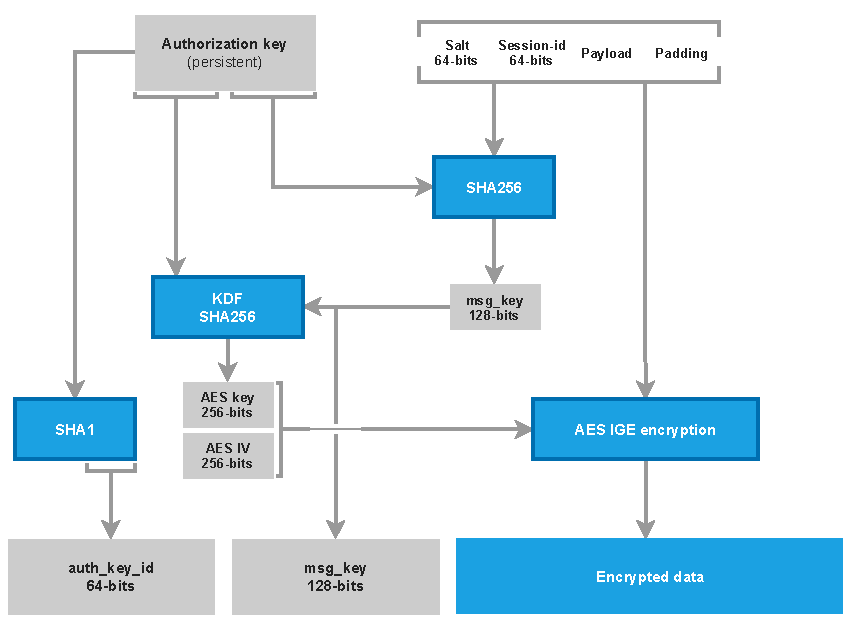
\includegraphics{cloud-chats}
  \caption{MTProto2.0 \cchat{} protocol.\\Representation inspired by the Telegram's official one.}
  \label{fig:cloud-chat-protocol}
\end{figure}
\begin{figure}[t]
  \centering
  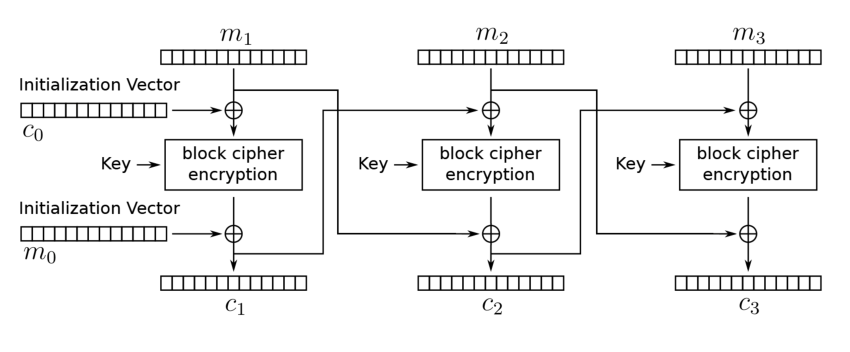
\includegraphics[width=.8\textwidth]{IGE}
  \caption{Encryption in IGE mode.}
  \label{fig:IGE}
\end{figure}

Telegram uses the schema in \cref{fig:cloud-chat-protocol} to encrypt every message exchanged between the client and the server after an authorization key has been established using the authorization protocol in \cref{sec:auth-prot}.

A message key msg\_key of 128 bits is calculated as the middle 128 bits of the SHA256 of the entire message prepended by 32 bytes of the authorization key. The message itself contains a 64-bit salt, a 64-bit session identifier, the payload\footnote{The payload contains the time of the message, its length, a sequence number. The receiver should check these pieces of information after decryption.} and a variable size padding of 12-1024 bytes.
The authorization key auth\_key, combined with the message key msg\_key, is used to derive a key and an initialization vector, which are used to encrypt the entire message using AES in IGE mode.

\subsection{IGE mode}
Infinite Garble Extension (in short, IGE) is a block cipher mode, lesser-known than others like ECB, CBC, OFB, CTR, CFB, GCM, CCM.
IGE can be defined with the following formula:

\begin{equation}
  c_i = f_K(m_i \oplus c_{i-1}) \oplus m_{i-1}
\end{equation}

where $f_K$ stands for the encrypting function (like AES) with key $K$
and $i$ goes from 1 to $n$ (the number of plaintext blocks). Two initialization vectors, $c_0$ and $m_0$, are also needed. \Cref{fig:IGE} summarizes how the encryption in IGE mode works.


One of the main properties of IGE mode is that it makes sure that if a ciphertext block is changed, then every subsequent block following it will not decrypt correctly.

As pointed out by \cite{Telegram-AFAQ-IGE}, the Telegram developers team is aware of the vulnerability of this mode to blockwise-adaptive Chosen Plaintext Attack (CPA)\cite{IGE-CPA}, but they claim that MTProto2.0 is not affected.




\section{\Schat{} protocol}
\label{sec:secret-chat}

Telegram's \schats{} deal with end-to-end encryption between two clients (as usual, let us call the clients Alice and Bob, or A and B for brevity). After both clients have shared an authorization key with the Telegram server S, they can decide to engage themselves in a run of the \schat{} protocol, allowing them to share, using a \DiHe{} key exchange, a common secret. Notice that the server acts as a forwarder: every message sent from a client A to another client B is sent to the server, encrypted as a \cchat{} message shown in \cref{sec:cloud-chat} with the authorization key of A; the server then decrypts the message and encrypts it as a \cchat{} message using the authorization key of B and finally sends it to B. The writing $\enc{M}{\key{AS}}$ in \cref{fig:secret-chat-protocol} expresses that the message $M$ has been encrypted with the authorization key $\key{AS}$ using the \cchat{} encryption schema \cref{sec:cloud-chat}.

%% Secret-chat protocol %%
\begin{figure}[!t]
  \setlength{\instdist}{3cm}
  \setmscoptions
  \begin{msc}{}
    \setmscscale{.8}

    \declinst{alice}{}{Alice}
    \declinst{server}{}{Server}
    \declinst{bob}{}{Bob}

    % Initial knowledge (auth keys)
    \action*{Knows $\key{AS}, \key{BS}$}{server}
    \action*{Knows $\key{AS}$}{alice}
    \action*{Knows $\key{BS}$}{bob}

    \nextlevel[3]
    \mess{$\enc{\func{getDhConfig}{}}{\key{AS}}$}{alice}{server}
    \nextlevel[2]
    \mess{$\enc{g, p}{\key{AS}}$}{server}{alice}
    \nextlevel

    \action*{\parbox{4cm}{\centering
        Generates $sID$\\
        $a \in \group{p}$\\
        $g_a := \modexp{g}{a}{p}$
      }}{alice}

    \nextlevel[5]

    %% TODO: Telegram webpage does not seem to specify HOW this is encrypted!!
    %% UPDATE: It actually (kinda) does: it's encrypted as a cloud-chat message! For simplicity, keep this notation and explain its meaning in the written part.
    \mess{$\enc{sID, B, g_a}{\key{AS}}$}{alice}{server}
    \nextlevel
    \mess{$\enc{sID, B, A, g_a}{\key{BS}}$}{server}{bob}
    \nextlevel[2]
    \mess{$\enc{\func{acceptChat}{}}{\key{BS}}$}{bob}{server}
    \nextlevel[2]
    \mess{$\enc{g, p}{\key{BS}}$}{server}{bob}
    \nextlevel

    \action*{\parbox{4cm}{\centering
        $b \in \group{p}$\\
        $g_b := \modexp{g}{b}{p}$\\
        $\key{AB} := \modexp{g_a}{b}{p}$
      }}{bob}

    \nextlevel[5]
    \mess{$\enc{sID, g_b, \sha{1}{k_{AB}}}{\key{BS}}$}{bob}{server}
    \nextlevel
    \mess{$\enc{sID, B, g_b, \sha{1}{k_{AB}}}{\key{AS}}$}{server}{alice}
    \nextlevel

    \action*{\parbox{4cm}{\centering
        $\key{AB} := \modexp{g_b}{a}{p}$\\
        Generates $msg$
      }}{alice}

    \nextlevel[3]
    \condition{Out-of-band $\key{AB}$ fingerprint comparison}{alice,server,bob}
    \nextlevel[4]
    \mess{$\enc{\enc{msg}{\key{AB}}}{\key{AS}}$}{alice}{server}
    \nextlevel
    \mess{$\enc{\enc{msg}{\key{AB}}}{\key{BS}}$}{server}{bob}

  \end{msc}

  \centering
  \caption{MTProto2.0 \Schat{} protocol}
  \label{fig:secret-chat-protocol}
\end{figure}

Let us describe the protocol steps, which are summed up in \cref{fig:secret-chat-protocol}. We will examine a run where Alice requests the \schat{}. Notice that we assume that both Alice and Bob have already exchanged an authorization key with the server ($\key{AS}$ and $\key{BS}$, respectively).

\begin{enumerate}
  \item{First of all, client A retrieves \DiHe{} parameters ($p, g$) from the server. Then, it generates a \DiHe{} ephemeral key $a$ and a session identifier $sID$. Finally, it computes his \DiHe{} half key $g_a:= \modexp{g}{a}{p}$ and sends $\left<sID, B, g_a\right>$ to client B;}
  \item{Client B receives the \schat{} request and may either accept it or deny it. Upon accepting it, it receives $p, g$, generates his ephemeral key $b$, computes his half key $g_b:= \modexp{g}{b}{p}$ and the newly created \schat{} key $\key{AB}:= \modexp{g_a}{b}{p}$. Lastly, it sends $\left<sID, g_b, \sha{1}{\key{AB}}\right>$ to client A. The hash function performed on the key is, as stated in the official documentation, only used as a sanity check for client developers;}
  \item{Client A receives the half key of B $g_b$ and uses it to compute the \schat{} key $\key{AB}:= \modexp{g_b}{a}{p}$. If the fingerprint of the key matches the one sent by B, it accepts the \schat{} and can start sending and receiving messages\footnote{The encryption schema used to encrypt end-to-end messages is very similar to the \cchat{} schema. We will not report it for brevity. The main difference is in the composition of the message. Please refer to \cite{Telegram-EndToEnd} for more details.}.}
\end{enumerate}

Mind that \DiHe{} generator ($g$), ephemeral keys ($a, b$) and half keys ($g_a, g_b$) are supposed to be checked by the clients as shown in \cref{item:DH-clients-checks}. Additionally, they should check all these values are greater then $1$ and smaller then $p-1$. Telegram team also recommends to check that $2^{2048}\leq g_a, g_b \leq \left(p-2\right)^{2064}$.

Notice that, as this exchange lacks authentication of the two clients, a compromised server can trivially perform a classic \DiHe{} \mitm{} attack \cite{DH-MITM}. To this end, Telegram requires the clients to check if their key fingerprints match. This must be done in an authenticated way using an out-of-band channel (e.g. in-person). This comparison is a necessary condition to ensure secrecy in further exchanges between participating clients.

\section{Rekeying protocol}
\label{sec:rekeying}

%% Rekeying protocol %%
\begin{figure}[t]
  \setlength{\instdist}{3.5cm}
  \setmscoptions
  \begin{msc}{}
    \setmscscale{.8}

    \declinst{alice}{}{Alice}
    \declinst{server}{}{Server}
    \declinst{bob}{}{Bob}

    % Initial knowledge (auth keys)
    \action*{Knows $\key{AS}, \key{BS}$}{server}
    \action*{Knows $\key{AS}, \key{AB}, p, g$}{alice}
    \action*{Knows $\key{BS}, \key{AB}, p, g$}{bob}

    \nextlevel[2]
    \action*{\parbox{4cm}{\centering
        Generates $eID$\\
        $a \in \group{p}$\\
        $g_a := \modexp{g}{a}{p}$
      }}{alice}

    \nextlevel[6]
    \mess{$\enc{\enc{eID, g_a}{\key{AB}}}{\key{AS}}$}{alice}{server}
    \nextlevel
    \mess{$\enc{\enc{eID, g_a}{\key{AB}}}{\key{BS}}$}{server}{bob}
    \nextlevel

    \action*{\parbox{4cm}{\centering
        $b \in \group{p}$\\
        $g_b := \modexp{g}{b}{p}$\\
        $\newkey{AB} := \modexp{g_a}{b}{p}$
      }}{bob}

    \nextlevel[6]
    \mess{$\enc{\enc{eID, g_b, \sha{1}{\newkey{AB}}}{\key{AB}}}{\key{BS}}$}{bob}{server}
    \nextlevel
    \mess{$\enc{\enc{eID, g_b, \sha{1}{\newkey{AB}}}{\key{AB}}}{\key{AS}}$}{server}{alice}
    \nextlevel

    \action*{\parbox{4cm}{\centering
        $\newkey{AB}:= \modexp{g_b}{a}{p}$
      }}{alice}

    \nextlevel[4]
    \mess{$\enc{\enc{eID, \sha{1}{\newkey{AB}}}{\key{AB}}}{\key{AS}}$}{alice}{server}
    \nextlevel
    \mess{$\enc{\enc{eID, \sha{1}{\newkey{AB}}}{\key{AB}}}{\key{BS}}$}{server}{bob}

  \end{msc}

  \centering
  \caption{MTProto2.0 Rekeying protocol}
  \label{fig:rekeying-protocol}
\end{figure}

This protocol is used to enable \pfs{} in \schats{}. Clients compliant with the protocol specification are supposed to initiate rekeying once a \schat{} key has been used to encrypt and decrypt more than 100 messages, or it has been in use for at least a week (and was used at least once). Any client participating in a \schat{} can start a run of the rekeying protocol.

Rekeying is based on \DiHe{}, which ensures that access to old keys does not grant knowledge of new ones. Moreover, the exchange is encrypted with the \schat{} key shared between clients, which effectively authenticates clients under the assumption of secrecy of the key itself. Under the premise of secrecy of the initial \schat{} key, this also rules out the possibility of a \mitm{} attack executed by a compromised server.

Let us examine the rekeying protocol, represented schematically in \cref{fig:rekeying-protocol}. We assume that clients engaging the rekeying protocol have already shared a \schat{} key $\key{AB}$. In addition, clients re-use \DiHe{} parameters $p, g$ obtained from the previous \schat{} protocol run.

\begin{enumerate}
  \item{Client A generates its \DiHe{} ephemeral key $a$ and an exchange identifier $eID$. Then, it computes its half key $g_a:= \modexp{g}{a}{p}$ and sends $\left<eID, g_a\right>$ to client B;}
  \item{Client B receives A's half key $g_a$, generates its own ephemeral key $b$ and computes the corresponding half key $g_b:= \modexp{g}{b}{p}$, as well as the new key $\newkey{AB}:= \modexp{g_a}{b}{p}$. Lastly, it sends $\left<eID, g_b, \sha{1}{\newkey{AB}}\right>$ to client A. As it was for the \schat{} protocol, the hash function performed on the new key is only used as a sanity check for client developers;}
  \item{Client A receives the half key of B $g_b$ and uses it to compute the new key $\newkey{AB}:= \modexp{g_b}{a}{p}$. After checking the hash, it sends the last message (basically an acknowledgement) containing $\left<eID, \sha{1}{\newkey{AB}}\right>$.}
\end{enumerate}

\chapter{Formalization in Tamarin prover}
In this section, we will explore the implementation of the MTProto2.0 protocol created in Tamarin prover. The full code is available on GitHub \cite{MTProto2-Tamarin}. Please refer to the README instructions for the code structure and for how to run the code.

This formalization is based on the paper \cite{MTProto2-Proverif} and the Proverif analysis \cite{MTProto2-Proverif-impl} of MTProto2.0 by \MMNV{}.

We will proceed to analyze the implementation of every single protocol and schema described in \cref{sec:mtproto2-informal}.

\section{Authorization protocol}
\label{sec:auth-prot-formalization}
\subsection{Exchanges formalization}
Let us describe how the protocol was formalized. See \cref{fig:formalization-authorization-protocol} for the updated schematic of the protocol.

%% Authorization protocol %%
\begin{figure}[!t]
  \setlength{\instdist}{4cm}
  \setmscoptions
  \begin{msc}{}
    \setmscscale{.8}

    \declinst{client}{}{Client}
    \declinst{server}{}{Server}

    \action*{Generates nonces $n_{c}, n_{k}$}{client}
    \action*{\parbox{4.5cm}{\centering
        Knows keys $\mbox{sk}^{(1)}, \dots, \mbox{sk}^{(n)}$\\
        Generates $n_s$
      }}{server}
    \nextlevel[4]

    \mess{$n_{c}$}{client}{server}
    \nextlevel[2]
    \mess{$n_{c}, n_{s}, \mbox{fp}^{(x)}$}{server}{client}

    \nextlevel
    \action*{\parbox{4cm}{\centering
        Gets $\mbox{pk}^{(x)}$ using $\mbox{fp}^{(x)}$\\
        $C_1 := n_c, n_s, n_k$
      }}{client}

    \nextlevel[5]
    \mess{$n_c, n_s, \mbox{fp}^{(x)}, \enc{C_1}{\mbox{pk}^{(i)}}$}{client}{server}
    \nextlevel

    \action*{$\left(k, iv\right) := \func{genKey}{n_s, n_k}$}{client}
    \action*{\parbox{4.5cm}{\centering
        Generates $s$\\
        $g_s := g^s$\\
        $key, iv := \func{genKey}{n_s, n_k}$\\
        $S_1 := n_c, n_s, g_s$
      }}{server}

    \nextlevel[6]
    \mess{$n_c, n_s, \enc{S_1}{key, iv}$}{server}{client}
    \nextlevel

    \action*{\parbox{4.5cm}{\centering
        Generates $c$\\
        $g_c := g^c$\\
        $\key{CS} := g_s^c$\\
        $C_2 := n_c, n_s, g_c$
      }}{client}
    \nextlevel[7]

    \mess{$n_c, n_s, \enc{C_2}{k, iv}$}{client}{server}
    \nextlevel

    \action*{\parbox{4.5cm}{\centering
        $\key{CS} := g_c^s$
      }}{server}
    \nextlevel[3]

    \mess{$n_c, n_s, \hash{n_k, \key{CS}}$}{server}{client}
  \end{msc}
  \centering
  \caption{MTProto2.0 Authorization protocol (simplified)}
  \label{fig:formalization-authorization-protocol}
\end{figure}

\lstset{language=tamarin}

\paragraph{Round 1}
Client nonces (both $n_c$ and $n_k$) are generated as fresh terms.
\DiHe{} parameters ($p$ and $g$) are not modeled: instead, we use a single public constant \lstinline{'g'} that represents the generator. In Tamarin, this is needed to avoid having lots of partial deconstructions, which were causing the non-termination of the protocol proofs. As this public constant is known to everyone (including the attacker), there is no need to send it to the client in \nth{4} message. This simplification makes even more sense if we consider that MTProto2.0 uses only six values for the generator $g$ ($2, 3, 4, 5, 6, 7$).

Moreover, the proof-of-work is not included as we are dealing with the protocol in a symbolic model. Finally, in our formalization, we assume that the client is able to get the public key of the server from its fingerprint. In Telegram, these keys are usually embedded in the application itself, resulting in the possibility of tampering \cite{MTProto2-Proverif}. Keypairs are generated using the following rule:

\begin{lstlisting}
rule RegisterPublicKey:
  let
    pkey        = pk(~skey)
    fingerprint = fpk(pkey)
  in
    [ Fr(~skey) ]
  -->
    [ !PrivateKey($X, ~skey), !PublicKey($X, pkey, fingerprint), Out(pkey) ]
\end{lstlisting}

In particular, the server decides which public key to use beforehand. Hence, a single key fingerprint is sent to the client. As the attacker cannot add its keys, this does not affect the soundness of the results.

\paragraph{Round 2} Another simplification is seen in the \nth{3} message: as encryption is not malleable in the symbolic model, there is no need to introduce the hash of the plaintext message along with the message itself. Notice that this hash was used as a Message Authentication Code (MAC) to check data integrity after decryption. This applies to every message from now on. Public key encryption is defined using the built-in \lstinline{asymmetric-encryption} equational theory.

Following from the formalization in Proverif, we do not model time, and the generic key derivation function $\kdf{}$ has been renamed to $\func{genKey}{}$. Lastly, a public constant \lstinline{'StoC'} (\lstinline{'CtoS'}) has been used to mark the message from the server to the client (from the client to the server) that contains the server (client) \DiHe{} half key. This is needed to avoid adding an incorrect reflection attack in which the server receives the message he has previously sent. In reality, the encryption actually contains some data that allows matching messages. Symmetric encryption is modeled using the built-in \lstinline{symmetric-encryption} equational theory.

\lstset{language=tamarin}
In the implementation, we also make substantial usage of pattern matching. Besides, using pattern matching is encouraged by Tamarin's manual as it usually decreases partial deconstructions. We have made use of it to ensure that half keys of client and server are actually in the form of \lstinline{'g'^~x}. This trick improves verification times by a lot, while it leaves the \mitm{} attack still possible\footnote{The attacker only needs to use its own ephemeral key and send the corresponding half key.}. We will use this modeling trick for every \DiHe{} exchange, including the one used in the \schat{} and rekeying protocols.

\paragraph{Round 3} No simplification is needed for the last round, except for removing the $retryID$, meaning that we assume that the exchange is always successful. Notice that this is consistent with the MTProto2.0 specification: the client needs to retry to send his half key only when the server finds a duplicated key hash, but, in our model, this never happens as client and server use fresh values as \DiHe{} ephemeral keys.

\subsection{Additional implementation notes}
Every encrypted exchange is tagged with a public constant \lstinline{'AUTH_X'}, which should improve efficiency.

The server's nonce in the model might also be fixed, which models a flawed server implementation or a server lacking randomness. The following rules are used to achieve this behavior:

\begin{lstlisting}
rule GenerateRandomServerNonce:
    [ Fr(~ns) ]
  -->
    [ NS(~ns) ]

rule GenerateFixedServerNonce:
    []
  -->
    [ NS('FIXED_NS') ]
\end{lstlisting}

The server then, in the multiset rewriting rule premises, uses the \lstinline{NS(ns)} fact.

Finally, many compromise rules are created:
\begin{itemize}
  \item Compromise of server long-term key (asymmetric private key)
  \item Compromise of client secret nonce $n_k$
  \item Compromise of server ephemeral key (DH exponent)
  \item Compromise of client ephemeral key (DH exponent)
  \item Compromise of authorization keys
\end{itemize}

As compromise rules are very simple and similar to each other, we will only show an example:

\begin{lstlisting}
/* Reveals the client's DH secret exponent. */
rule CompromiseAuthProtClientExponent:
    [ !AuthProtClientEphemeralSecrets(nk, c) ]
  --[ CompromisedClientExponent(c) ]->
    [ Out(c) ]
\end{lstlisting}

Using these compromise rules, we can also check if the protocol is secure in the eCK model \cite{eCK}. The eCK model assumes, in the case of an authenticated key exchange, two parties, each having a long-term and an ephemeral secret. Of these four pieces of information, the eCK model allows revealing any subset that does not contain both long-term and ephemeral secrets.
In MTProto2.0, the authorization protocol does not respect the eCK model as the client has no long-term secret. Moreover, intuitively, we can already notice that the protocol is not secure in the eCK model: revealing the client ephemeral secret $n_k$ allows the attacker to perform a classic \mitm{} attack on the \DiHe{} exchange \cite{MITM-DH}.

\subsection{Security properties verification}
Every rule in the protocol execution is labeled with action facts. We then use these to model security properties. Following the Proverif formalization, we have modeled several forms of key agreement, authentication of parties and key secrecy, along with observational equivalence queries on the secret nonce $n_k$ and the authorization key. In the following paragraphs, we are going to examine lemmas and related results in more detail.

\paragraph{Key agreement}
The following lemma models key agreement:
\begin{lstlisting}[numbers=left]
lemma LemmaAuthProtAgreement:
  "
    /* Whenever a client and a server negotiate an authorization key */
    ∀ nc ns nk authKey1 authKey2 #i #j.
      (
        ServerAcceptsAuthKey(nc, ns, nk, authKey1) @i ∧
        ClientAcceptsAuthKey(nc, ns, nk, authKey2) @j ∧

        /* and no secret was leaked */
        ¬(∃ sk #r.   CompromisedAuthKey(sk) @r) ∧
        ¬(∃ skey #r. CompromisedPrivateKey(skey) @r) ∧
        ¬(∃ n #r.    CompromisedNk(n) @r) ∧
        ¬(∃ c #r.    CompromisedClientExponent(c) @r) ∧
        ¬(∃ s #r.    CompromisedServerExponent(s) @r)
      )
      ==>
      (
        /* then the authorization key is the same */
        ( authKey1 = authKey2 ) ∨
        
        /* 
         * or the server is actually running two different instances
         * of the protocol with the client
         */
        (
          ∃ #n1 #n2.
            ServerGeneratesNonce(ns) @n1 ∧
            ServerGeneratesNonce(ns) @n2 ∧
            ¬(#n1 = #n2)
        )
      )
  "
\end{lstlisting}

By commenting any line between 10-14 (inclusive), we can model agreement in the presence of some information leakage.
Key agreement without leaks holds. It may be interesting to notice that key agreement holds even when both ephemeral keys are revealed as the attacker cannot force the client and the server to compute different keys. Compromising one at a time either server's private key or client nonce allows the attacker to execute a \mitm{} attack on the \DiHe{} exchange.

We can also prove a similar property: if a client and a server end a run of the protocol negotiating the same key in their unrelated sessions, then these sessions actually coincide.

\paragraph{Authentication}
Client authentication in the protocol does not hold because the client does not authenticate itself and the server is willing to execute the protocol with anybody (including the attacker). This query captures this:

\begin{lstlisting}
lemma LemmaAuthProtAuthClientToServer:
  "
    ∀ nc ns nk authKey #i #j.
      /* Whenever a client has started a session with nonce nc */
      ClientStartsSession(nc) @i ∧

      /* and the server has sent an ACK for the session <nc, ns> */
      ServerSendsAck(nc, ns, nk, authKey) @j ∧

      /* and no secret was leaked */          
      ¬(∃ sk #r.   CompromisedAuthKey(sk) @r) ∧
      ¬(∃ skey #r. CompromisedPrivateKey(skey) @r) ∧
      ¬(∃ n #r.    CompromisedNk(n) @r) ∧
      ¬(∃ c #r.    CompromisedClientExponent(c) @r) ∧
      ¬(∃ s #r.    CompromisedServerExponent(s) @r)
      ==>
      (
        /* then a client has shared an authKey with the server */
        (
          ∃ #k.
          ClientAcceptsAuthKey(nc, ns, nk, authKey) @k
        ) ∨

        /* 
         * or the server is actually running two different instances
         * of the protocol with the client
         */
        (
          ∃ #k #l.
            ServerGeneratesNonce(ns) @k ∧
            ServerGeneratesNonce(ns) @l ∧
            ¬(#k = #l)
        )
      )
  "
\end{lstlisting}

However, we can prove the server knows that the client that negotiated the authorization key is the same that sends the third message. For the sake of brevity, we will not report the related lemma. As anyone can create an authorization key with the server, this lack of authentication is not an issue.

However, server authentication is fundamental, and it is captured by the following lemma:
\begin{lstlisting}[numbers=left]
  lemma LemmaAuthProtAuthServerToClient:
    "
      ∀ nc ns nk authKey #i1.
        /* Whenever a client receives an ACK from the server */
        ClientReceivesAck(nc, ns, nk, authKey) @i1 ∧
        
        /* and no secret was leaked */
        ¬(∃ sk #r.   CompromisedAuthKey(sk) @r) ∧
        ¬(∃ skey #r. CompromisedPrivateKey(skey) @r) ∧
        ¬(∃ n #r.    CompromisedNk(n) @r) ∧
        ¬(∃ c #r.    CompromisedClientExponent(c) @r) ∧
        ¬(∃ s #r.    CompromisedServerExponent(s) @r)
        ==>
        (
          /* then there is a session matching it on the server */
          ( 
            ∃ #j.
            ServerAcceptsAuthKey(nc, ns, nk, authKey) @j ∧
            (∀ #i2. ClientReceivesAck(nc, ns, nk, authKey) @i2 ==> #i1 = #i2)
          ) ∨

          /* or the server has reused the same nonce */
          (
            ∃ #j1 #j2.
              ServerGeneratesNonce(ns) @j1 ∧
              ServerGeneratesNonce(ns) @j2 ∧
              ¬(#j1 = #j2)
          )
        )
    "
\end{lstlisting}

This lemma holds, meaning that the server is authenticated to the client. Notice that line 19 models injectivity.

\paragraph{Key secrecy}
Another fundamental property of the authentication protocol is key secrecy: when a client and a server negotiate a key, they must be sure that the key is known only to them. This property is proved using the following lemma:
\begin{lstlisting}
lemma LemmaAuthProtKeySecrecy:
  "
    /* Whenever client and server negotiated a key */
    ∀ nc ns nk authKey #i #j #k.
      ClientAcceptsAuthKey(nc, ns, nk, authKey) @i ∧
      ServerAcceptsAuthKey(nc, nk, nk, authKey) @j ∧

      /* and the attacker knows it */
      K(authKey) @k
      ==>
      /* then some secret was leaked */
      (
        (∃ #r.      CompromisedAuthKey(authKey) @r) ∨
        (∃ skey #r. CompromisedPrivateKey(skey) @r) ∨
        (∃ #r.      CompromisedNk(nk) @r) ∨
        (∃ c #r.    CompromisedClientExponent(c) @r) ∨
        (∃ s #r.    CompromisedServerExponent(s) @r)
      )

  "
\end{lstlisting}

\paragraph{Observational equivalence}
Attempts to prove observational equivalence for client's secret nonce $n_k$ and authorization key, unfortunately, do not terminate. Notice that observational equivalence is often extremely resource-consuming.

Observational equivalence in Tamarin is expressed using the \lstinline{diff/2} operator, which duplicates every rule, one for the left-hand side and one for the right-hand side of the operator, and tries to find a difference between the two traces.

In the formalization, we created the two following rules:

\newpage

\begin{lstlisting}
/*
 * The secret nonce nk generated by the client is indistinguishable 
 * from a fresh value.
 */
rule RuleAuthProtNkEquivalence:
    [
      !AuthProtClientEphemeralSecrets(nk, b),
      Fr(~n)
    ]
  -->
    [ Out(diff(nk, ~n)) ]

/*
 * A negotiated authorization key authKey is indistinguishable from a 
 * fresh value.
 */
rule LemmaAuthProtAuthKeyEquivalence:
    [
      !AuthKeyClient(server, authKey),
      Fr(~freshAuthKey)
    ]
  -->
    [ Out(diff(~freshAuthKey, authKey)) ]
\end{lstlisting}





\section{\Cchat{} encryption schema}
\label{sec:cloud-chat-formalization}

\subsection{Encryption formalization}
\Cchat{} encryption has been simplified to suit the symbolic model better.
First of all, the key derivation function returns only the key. Notice that, as both key and initialization vector are derived from the same terms, once the adversary is able to compute the key it would be able to compute the IV as well. Hence, it is not modeled as it would only add complexity to the model without bringing any benefit.

A function \lstinline{msgKey/2} is used to create the message key from the message and the authorization key. Then, the message key is used to create the encryption key for the message, together with the authorization key, using the \lstinline{genKey/2} primitive. The plaintext message is encrypted using the built-in \lstinline{symmetric-encryption}. The final message that is sent on the channel is composed of the fingerprint of the authorization key (using \lstinline{keyID/1}), the message key and the encrypted message. Notice that functions \lstinline{msgKey/2}, \lstinline{genKey/2} and \lstinline{keyID/1} have no associated equation (i.e. are considered perfect hashing functions).

Four different rules have been created: two are used to exchange messages from client to server and the other two for messages from the server to the client. This approach allows us to test for secrecy in both directions. Here is an example of the rule used to model a client to server message:

\begin{lstlisting}
  rule ClientCloudChatSendsMessage:
    let
      msg = <'CC_CtoS', ~sessionID, ~m>
      mk  = msgKey(msg, authKey)
      key = genKey(mk, authKey)
      c   = <keyID(authKey), mk, senc(msg, key)>
    in
      [
        !AuthKeyClient($Server, authKey),
        Fr(~sessionID),
        Fr(~m)
      ]
    --[ ClientSendsCloudMessage(~sessionID, ~m, authKey) ]->
      [ Out(c) ]
\end{lstlisting}

Notice on line 3 that we use a public constant \lstinline{'CC_CtoS'} to differentiate client to server from server to client messages.

\subsection{Security properties verification}

\paragraph{Secrecy and forward secrecy} The \cchat{} encryption schema is essentially employed to obtain secrecy on messages exchanged between a client and a server after they have negotiated an authorization key.
The following lemma proves secrecy from client to server. A similar one is used to verify secrecy of messages from server to client.

\begin{lstlisting}
lemma LemmaCloudChatSecrecyClientToServer:
  "
    ∀ sid msg authKey #i #j #r.
      (
        /* Whenever a client sends a cloud message to the server */
        ClientSendsCloudMessage(sid, msg, authKey) @i ∧

        /* and the server receives it */
        ServerReceivesCloudMessage(sid, msg, authKey) @j ∧

        /* and the attacker knows it */
        K(msg) @r
      )
      ==>
      (
        /* then some secret was compromised */
        (∃ #r.      CompromisedAuthKey(authKey) @r) ∨
        (∃ skey #r. CompromisedPrivateKey(skey) @r) ∨
        (∃ n #r.    CompromisedNk(n) @r) ∨
        (
          (∃ c #r.   CompromisedClientExponent(c) @r) ∧
          (∃ s #r.    CompromisedServerExponent(s) @r)
        )
      )
  "
\end{lstlisting}

This lemma means that messages are secure, unless:
\begin{itemize}
  \item The private key of the server is compromised;
  \item The secret nonce $n_k$ of the client is compromised;
  \item \DiHe{} exponents of both client and server are compromised.
\end{itemize}

As seen in \cref{sec:auth-prot-formalization}, compromising any of these secrets leads to a lack of secrecy on the key. Additionally, the key itself can be compromised to break \cchats{} secrecy.

As the lemma above is also strict (i.e. removing any action fact leads to an attack trace), this also means that \pfs{} does not hold in \cchats{} as an attacker that is able to compromise the authorization key can decrypt both past and future messages (as well as forging them, effectively impersonating the client to the server).






\section{\Schat{}}
\label{sec:secret-chat-formalization}
A \schat{} can be created after clients have both shared an authorization key with the server. To create a shared secret (the \textit{\schat{} key}) between two clients, MTProto2.0 uses, as already seen in \cref{sec:secret-chat}, a \DiHe{} key exchange in which the Telegram server acts as a forwarder.

As we have already analyzed the security of the authorization protocol and of the \cchat{} encryption in \cref{sec:auth-prot-formalization,sec:cloud-chat-formalization}, in the formalization we do not encrypt messages with the authorization key, nor we use the server as a forwarder. Instead, we execute the \schat{} protocol exchanges as if they were plaintext: this allows the attacker to act as the server (i.e. having knowledge of both authorization key and forwarding messages) and to manipulate messages \cite{MTProto2-Proverif}. Additionally, removing this layer of encryption allows simplifying the protocol model, formulating stronger security properties, and obtaining better efficiency. For these reasons, we do not model any rule that creates dummy authorization keys nor execute the authorization protocol to obtain them.

\subsection{Exchanges formalization}
%% Secret-chat protocol %%
\begin{figure}[!t]
  \setlength{\instdist}{3cm}
  \setmscoptions
  \begin{msc}{}
    \setmscscale{.8}

    \declinst{alice}{}{Alice}
    \declinst{bob}{}{Bob}

    \action*{\parbox{3.5cm}{\centering
        Knows $\key{AS}$\\
        Knows $g$\\
        Generates $sID, a$\\
        $g_a := g^a$
      }}{alice}
    \action*{Knows $\key{BS}$}{bob}

    \nextlevel[7]
    \mess{$sID, A, B, g_a$}{alice}{bob}
    \nextlevel

    \action*{\parbox{3.5cm}{\centering
        Knows $g$\\
        Generates $b$\\
        $g_b := g^b$\\
        $\key{AB} := g_a^b$
      }}{bob}

    \nextlevel[6]
    \mess{$sID, A, B, g_b, \func{fps}{k_{AB}}$}{bob}{alice}
    \nextlevel

    \action*{\parbox{4cm}{\centering
        $\key{AB} := g_b^a$\\
        Generates $msg$
      }}{alice}

    \nextlevel[3]
    \condition{Out-of-band $\key{AB}$ fingerprint comparison}{alice,bob}
    \nextlevel[4]
    \mess{$\enc{msg}{\key{AB}}$}{alice}{bob}

  \end{msc}

  \centering
  \caption{MTProto2.0 \Schat{} protocol formalization}
  \label{fig:secret-chat-protocol-formalization}
\end{figure}

Following the Proverif formalization, we explicitly name clients and allow the attacker to choose their roles (i.e. who the initiator is, whom the initiator talks to, who the responder is). We apply restriction rules to ensure that the initiator is always honest:

\newpage

\begin{lstlisting}
restriction RestrictionChoosePrincipal:
  "
    ∀ X Y Z #i.
      ChoosePrincipal(X, Y, Z) @i ==> ((X = Y) ∨ (X = Z))
  "
\end{lstlisting}

However, the responder may as well be a dishonest party. Having named clients explicitly, we can prove additional authentication security properties.

Finally, we model the QR-code comparison with the following rules:

\begin{lstlisting}
rule PerformOutOfBandKeyComparison:
    [ 
      !QR(aID, aUser, bUser, sessionKey),
      !QR(bID, bUser, aUser, sessionKey)
    ]
  --[ 
      /* Rule out the possibility of sessions of a client with itself */
      NotEq(aUser, bUser),

      OutOfBandKeyComparisonSucceeded(aID, aUser, bUser, sessionKey),
      OutOfBandKeyComparisonSucceeded(bID, bUser, aUser, sessionKey)
    ]->
    [
      !QROK(aID, aUser, bUser, sessionKey),
      !QROK(aID, bUser, aUser, sessionKey)
    ]

rule SkipOutOfBandKeyComparison:
    [ !QR(aID, aUser, bUser, sessionKey) ]
  --[ OutOfBandKeyComparisonSkipped(aID, aUser, sessionKey)]->
    [ !QROK(aID, aUser, bUser, sessionKey) ]

restriction RestrictionNotEqual:
  "∀ x y #i. NotEq(x, y) @i ==> ¬(x = y)"
\end{lstlisting}

The persistent fact \lstinline{!QR} is created by each party after they have computed the \schat{} key. The above rules model both the correct and incorrect behavior of clients, allowing to specify properties in which a specific behavior is taken. The correct behavior is the one express by the \lstinline{PerformOutOfBandKeyComparison} rule, where the client implicitly checks that the \lstinline{sessionKey} he computed is the same as the other party. The incorrect behavior in rule \lstinline{SkipOutOfBandKeyComparison} models a client that does not match the key fingerprint: as this is the only way of authenticating parties to each other, skipping the comparison may result in a \DiHe{} \mitm{} attack.

Additionally, two rules have been added to allow message sending and receiving:

\begin{lstlisting}
rule SecretChatSend:
  let
    mk  = msgKey(~m, sessionKey)
    key = genKey(mk, sessionKey)
    c   = <keyID(sessionKey), mk, senc(~m, key)>
  in
    [ 
      !SecretChatClient(X, iUser, rUser, xID, chatID, sessionKey, authKey),
      Fr(~m)
    ]
  --[
      ClientSendsSecretChatMsg(chatID, X, iUser, rUser, sessionKey, ~m)
    ]->
    [ Out(c) ]

rule SecretChatReceive:
  let
    mk  = msgKey(~m, sessionKey)
    key = genKey(mk, sessionKey)
    c   = <keyID(sessionKey), mk, senc(~m, key)>
  in
    [
      !SecretChatClient(X, iUser, rUser, xID, chatID, sessionKey, authKey),
      In(c)
    ]
  --[ ClientReceivesSecretChatMsg(chatID, X, iUser, rUser, sessionKey, ~m) ]->
    []
\end{lstlisting}

As already noted in \cref{sec:secret-chat}, the encryption schema for \schat{} messages slightly differs from the \cchat{} one. However, from a symbolic point of view, they are equivalent. Hence, we model the \schat{} encryption with the same steps described in \cref{sec:cloud-chat-formalization}.

\Cref{fig:secret-chat-protocol-formalization} shows the \schat{} protocol, with the simplifications described above.

\subsection{Security properties verification}

Two main properties should be satisfied by the \schat{} protocol: secrecy and authentication.


\paragraph{Secrecy} This is, of course, one of the most important properties for an end-to-end chat. MTProto2.0 guarantees secrecy under the assumption that clients compare the \schat{} key fingerprint out-of-band. This mechanism is also used, for example, by Signal \cite{SignalProtocol}. Formally, Tamarin is able to prove the following secrecy lemma:

\begin{lstlisting}
lemma LemmaSecretChatSecrecy:
  "
    /* Whenever the client sends a secret chat message msg */
    ∀ chatID X iUser rUser sessionKey msg #i #j.
      ClientSendsSecretChatMsg(chatID, X, iUser, rUser, sessionKey, msg) @i ∧
      
      /* but the attacker knows it */
      K(msg) @j
      ==>
      (
        /* then clients skipped the QR validation */
        ∃ a #r. OutOfBandKeyComparisonSkipped(a, X, sessionKey) @r
      )
  "
\end{lstlisting}

In other words, unless clients skipped the key fingerprint comparison, the exchanged messages are secret. Let us stress the fact that this result does not depend on the secrecy of the authorization key. Hence, if clients compare the fingerprint correctly, end-to-end encryption holds even against a compromised server.

\newpage
\paragraph{Authentication}
Many variants of authentication have been proven. The most generic one is the following:

\begin{lstlisting}
  lemma LemmaSecretChatAuthentication1:
  "
    /* Whenever a client received a secret chat message */
    ∀ chatID1 X iUser rUser msg sessionKey #i.
      ClientReceivesSecretChatMsg(chatID1, X, iUser, rUser, sessionKey, msg) @i
      ==>
      (
        /* then it was sent by another (honest) client */
        (∃ Y chatID2 #r. 
          ClientSendsSecretChatMsg(chatID2, Y, iUser, rUser, sessionKey, msg) @r) ∨
        (∃ Y chatID2 #r. 
          ClientSendsSecretChatMsg(chatID2, Y, rUser, iUser, sessionKey, msg) @r) ∨

        /* or clients involved have skipped the QR validation */
        (
          ∃ Y xID yID #r1 #r2. 
            OutOfBandKeyComparisonSkipped(xID, X, sessionKey) @r1 ∧
            OutOfBandKeyComparisonSkipped(yID, Y, sessionKey) @r2
        )
      )
  "
\end{lstlisting}

Notice that we cannot match sessions (i.e. $chatID1 = chatID2$) as the server can forward messages modifying the session identifier. As also pointed out by \MMNV{} \cite{MTProto2-Proverif}, this does not seem to pose any security risks.

As reported earlier, skipping QR comparison results in a classic \DiHe{} \mitm{} attack.

\paragraph{Observational equivalence} We have tried to model several observational equivalence properties, such as:
\begin{itemize}
  \item Indistinguishability of a client's exponent from a random value. This should not hold as the attacker can compute the DH key (using the exponent and the other half of the key) and compare fingerprints;
  \item Indistinguishability of a \schat{} key and a random value. This should not hold as the attacker can compare the key fingerprint with the \nth{2} message of the protocol;
  \item Indistinguishability of message exchanged with the \schat{} key and a random value. This should hold as long as the key used to encrypt the message is kept secret.
\end{itemize}

Again, Tamarin does not terminate when trying to prove these observational equivalences.



\newpage
\section{Rekeying}

%% Rekeying protocol %%
\begin{figure}[t]
  \setmscoptions
  \setlength{\instdist}{2.5cm}
  \begin{msc}{}
    \setmscscale{.8}

    \declinst{alice}{}{Alice}
    \declinst{bob}{}{Bob}

    \action*{Knows $\key{AB}, g$}{alice}
    \action*{Knows $\key{AB}, g$}{bob}

    \nextlevel[2]
    \action*{\parbox{3cm}{\centering
        Generates $eID, a$\\
        $g_a := g^a$
      }}{alice}

    \nextlevel[4]
    \mess{$\enc{eID, g_a}{\key{AB}}$}{alice}{bob}
    \nextlevel

    \action*{\parbox{3cm}{\centering
        Generates $b$\\
        $g_b := g^b$\\
        $\newkey{AB} := g_a^b$
      }}{bob}

    \nextlevel[5]
    \mess{$\enc{eID, g_b, \func{fps}{\newkey{AB}}}{\key{AB}}$}{bob}{alice}
    \nextlevel

    \action*{\parbox{3cm}{\centering
        $\newkey{AB}:= g_b^a$
        Generates $msg$
      }}{alice}

    \nextlevel[4]
    \mess{$\enc{eID, \func{fps}{\newkey{AB}}}{\key{AB}}$}{alice}{bob}
    \nextlevel[2]
    \mess{$\enc{msg}{\newkey{AB}}$}{alice}{bob}

  \end{msc}

  \centering
  \caption{MTProto2.0 Rekeying protocol formalization}
  \label{fig:rekeying-protocol-formalization}
\end{figure}

Finally, let us describe the rekeying protocol formalization, which allows \pfs{} on \schats{}.

\subsection{Exchanges formalization}
The formalization of the rekeying protocol is very similar to the formalization of the \schat{} protocol: we do not model the outer layer of encryption from client to server. The reasoning and implications are the same (see \cref{sec:secret-chat-formalization}).

The significant difference is that this time the \DiHe{} exchange is end-to-end encrypted using the \schat{} key exchanged (only) between clients. A schematic representation of the protocol's formalization is given in \cref{fig:rekeying-protocol-formalization}.

For efficiency and termination reasons, in our formalization the attacker can choose only the initiator's responder. Both initiator and responder are fixed. \Schat{} keys are generated using the following rules:

\newpage

\begin{lstlisting}
rule GenerateSecretChatKey:
  let
    X1 = 'Alice'
    X2 = 'Bob'
    sessionKey = 'g' ^ ~i ^ ~r
  in
    [
      Fr(~i),
      Fr(~r),
      Fr(~chatID)
    ]
  -->
    [ 
      !SecretChatClient(X1, X1, X2, ~i, ~chatID, sessionKey),
      !SecretChatClient(X2, X1, X2, ~r, ~chatID, sessionKey)
    ]

rule AttackerGeneratesSecretChatKey:
  let
    sessionKeyAlice = 'g' ^ ~e1 ^ ~e2
    sessionKeyBob = 'g' ^ ~e3 ^ ~e4
  in
    [ 
      Fr(~e1), Fr(~e2), Fr(~e3), Fr(~e4),
      Fr(~chatIDAlice), Fr(~chatIDBob)
    ]
  --[ AttackerRegisteredKey(sessionKeyAlice), AttackerRegisteredKey(sessionKeyBob) ]->
    [
      !SecretChatClient('Alice', 'Alice', 'Eve', ~e1, ~chatIDAlice, sessionKeyAlice),
      !SecretChatClient('Eve', 'Alice', 'Eve', ~e2, ~chatIDAlice, sessionKeyAlice),
      !SecretChatClient('Bob', 'Eve', 'Bob', ~e3, ~chatIDBob, sessionKeyBob),
      !SecretChatClient('Eve', 'Eve', 'Bob', ~e4, ~chatIDBob, sessionKeyBob),
      Out(<sessionKeyAlice, sessionKeyBob>)
    ]
\end{lstlisting}

The first models the generation for honest users, while the second allows the attacker to execute the protocol with honest users by creating a \schat{} with them and sharing the key with the attacker by outputting it. Notice that these rules implicitly assume the correctness of the \schat{} protocol, which we have proven in \cref{sec:secret-chat-formalization}.

A very important modelling decision has been taken, in order to achieve termination of lemmas: both initiator's and responder's first rule have a restriction \lstinline{OnlyTwice(x)}, where \lstinline{x} is \lstinline{'Initiator'} for initiator and \lstinline{'Responder'} for responder. The restriction is defined as follows:

\begin{lstlisting}
restriction RestrictionOnlyTwice:
  "
    ∀ x #i #j #k. 
      OnlyTwice(x) @i ∧
      OnlyTwice(x) @j ∧
      OnlyTwice(x) @k 
      ==>
      (
        #i = #j ∨
        #i = #k ∨
        #j = #k
      )
  "
\end{lstlisting}

This restriction allows only two instances of the \lstinline{OnlyTwice} fact (with the same argument) on the trace.
Nonetheless, this is the best solution that has been found to the non-termination problems observed during the modeling of this protocol\footnote{In essence, Tamarin was trying to gain knowledge of secret (i.e. exponents) or encrypted terms by executing the rekeying protocol many times with different \schat{} keys. This behavior appears to lead to non-termination.}. It is of the utmost importance to notice that this restriction may or may not compromise the soundness of results obtained in the verification process as it bounds the number of rekeying executions.

Message encryption is modeled as in \schats{} (see \cref{sec:secret-chat-formalization}).

\subsection{Security properties verification}
We would like to prove three properties: secrecy, \pfs{} and authentication.

\paragraph{Secrecy and \pfs{}}

Even in our scenario, it can be proven by Tamarin that secrecy holds after rekeying. The following lemma formalizes this property:

\begin{lstlisting}
lemma LemmaRekeyingMessageSecrecy:
  "
    /* There is no way two honest clients exchanged a message msg */
    ¬(∃ s r iUser rUser xID1 xID2 eID1 eID2 newKey msg #i1 #i2 #j.
      ClientSendsMessageWithNewKey(xID1, s, eID1, iUser, rUser, newKey, msg) @i1 ∧
      ClientReceivesMessageWithNewKey(xID2, r, eID2, iUser, rUser, newKey, msg) @i2 ∧

      /* and the attacker knows it */
      K(msg) @j
    )
  "
\end{lstlisting}

\Pfs{} is guaranteed by the periodic rotation of keys described in \cref{sec:rekeying}. We also proved that knowledge of authorization keys does not compromise secrecy.

\paragraph{Authentication}

\begin{figure}[t]
  \setmscoptions
  \setlength{\instdist}{2cm}
  \begin{msc}{}
    \setmscscale{.8}

    \declinst{alice}{}{Alice}
    \declinst{eve}{}{Eve}
    \declinst{bob}{}{Bob}

    \action*{Knows $\key{AE}, g$}{alice}
    \action*{Knows $\key{AE}, \key{BE}, g$}{eve}
    \action*{Knows $\key{BE}, g$}{bob}

    \nextlevel[2]
    \action*{\parbox{3cm}{\centering
        Generates $eID, a$\\
        $g_a := g^a$
      }}{alice}

    \nextlevel[4]
    \mess{$\enc{eID, g_a}{\key{AE}}$}{alice}{eve}
    \nextlevel
    \mess{$\enc{eID, g_a}{\key{BE}}$}{eve}{bob}
    \nextlevel

    \action*{\parbox{3cm}{\centering
        Generates $b$\\
        $g_b := g^b$\\
        $\newkey{AB} := g_a^b$
      }}{bob}

    \nextlevel[5]
    \mess{$\enc{eID, g_b}{\key{BE}}$}{bob}{eve}
    \nextlevel
    \mess{$\enc{eID, g_b}{\key{AE}}$}{eve}{alice}
    \nextlevel

    \action*{$\newkey{AB} := g_b^a$}{alice}

    \nextlevel[3]
    \mess{$\enc{eID, \func{fps}{\newkey{AB}}}{\key{AE}}$}{alice}{eve}
    \nextlevel
    \mess{$\enc{eID, \func{fps}{\newkey{AB}}}{\key{BE}}$}{eve}{bob}

  \end{msc}

  \centering
  \caption{\Uks{} attack on the rekeying protocol.}
  \label{fig:UKS}
\end{figure}

The other fundamental property of this protocol is the authentication of parties. Whenever two clients execute the rekeying protocol (successfully), they should be able to assume that the new key is known to both and only them.

The following lemma is used to verify that whenever two clients exchange the same key in the same session, there are only two (honest) parties involved:

\begin{lstlisting}
  lemma LemmaRekeyingAuthentication:
  "
    /* Whenever two users negotiate the same key in the same session */
    ∀ exchangeID iUser1 iUser2 rUser1 rUser2 newKey #i #j.
      InitiatorHasNegotiatedNewKey(exchangeID, iUser1, rUser1, newKey) @i ∧
      ResponderHasNegotiatedNewKey(exchangeID, iUser2, rUser2, newKey) @j
      ==>
      (
        /* then there are actually only two users involved */
        iUser1 = iUser2 ∨
        iUser1 = rUser2 ∨
        rUser1 = iUser2 ∨
        rUser1 = rUser2
      )
  "
\end{lstlisting}

However, Tamarin finds a counterexample for this lemma. Specifically, it finds the same attack described by \MMNV{}: an \textit{unknown key-share} attack.

Let A and E be two honest entities. This type of attack, defined by \SBWAM{} \cite{UKS}, allows a client A to believe it has shared a key with E, while it has instead shared it with B. In this particular case, this attack also compromises two other properties: \textit{implicit key confirmation} and \textit{implicit key authentication} \cite{MTProto2-Proverif}.
The first property states that client A is assured that the second entity B can compute the key. The latter states that client A is assured that no other entity, apart from B, can learn the value of the key \cite{UKS}.

Now, let us show how the attack unfolds in the following situation: assume there are three clients (A, B and E) and client E has already shared a \schat{} key. The steps of the attack are the following:

\begin{enumerate}
  \item A starts executing the rekeying protocol with E and E receives A's half key $g_a$;
  \item E now starts a concurrent execution with B using A's half key $g_a$ and obtains B's half key $g_b$. E may or may not reuse the same session identifier sent by A with B;
  \item E responds to A using B's half key $g_b$;
  \item A concludes the protocol run by sending the fingerprint of the new key. E then forwards, with the correct key, the fingerprint.
\end{enumerate}

As a result, client E neither uniquely possesses the key nor can compute it. \Cref{fig:UKS} shows a graphical representation of the attack.



\chapter{Comparison}
In this chapter, we will compare Tamarin prover and Proverif under several points of view.
In particular, the comparison is going to cover the following topics:
\begin{itemize}
    \item Usability
    \item Expressiveness
    \item Efficiency
    \item Soundness and completeness
\end{itemize}

\section{Usability}
This may be the most complex property to evaluate as perceived usability can change with different levels of expertise and previous backgrounds. Of course, a user who has already used the \pic{} and Prolog would probably feel more comfortable with Proverif's formalisms. The usability of these tools for the formal verification of cryptographic protocols is, in general, difficult to establish. To the best of our knowledge, no study has been published regarding this specific topic. Another issue regards the formalization in Proverif, which was created by \MMNV{}, meaning we cannot know the problems that arose during modeling.

As we have seen, Tamarin offers a wide variety of built-in cryptographic primitives. While these are not hard to define, having predefined primitives allows for faster modeling compared to Proverif (where every single primitive must be defined).

The labeled multiset rewriting rules used by Tamarin is also more "low-level" than the applied \pic{}. As such, modeling using the latter is usually easier. A variant of the applied \pic{}, Sapic, has also been created to allow protocol specification in a stateful version of the applied \pic{} which is then automatically translated to labeled multiset rewriting rules and analyzed using Tamarin \cite{kremer:hal-00955869}. The authors' intentions were to create a sound and complete verification tool that was not ``error-prone and difficult'' as Tamarin, while keeping its features intact \cite{sapic-website}.

The security properties of both languages should be straightforward to model as these are based on well-known logical constructs. However, the guarded fragment of first-order logic used by Tamarin has a more complex syntax, which can probably intimidate beginners at first.

Assuming no previous knowledge, we can conclude that Tamarin's formalism and language might be slightly more complex than Proverif's.

\section{Expressiveness}
The various built-in theories offered by Tamarin are also very expressive. As we have seen in \cref{sub:built-in-equational-theories}, the Diffie-Hellman, the xor, and the bilinear-pairing equational theories are modeled faithfully. Moreover, Tamarin is one of the few tools able to model exclusive or \cite{xor_tamarin}.

\lstset{language=proverif}
The labeled multiset rewriting rules used by Tamarin is a more low-level formalism than then applied \pic{}. Nonetheless, rewriting rules allow encoding stateful protocols, which are not supported by the \Horncs{} used by Proverif. Moreover, as reported by S. Kremer and K. Robert \cite{kremer:hal-00955869}, many other efficient tools, such as AVISPA \cite{10.1007/11513988_27} or Maude-NPA \cite{Escobar2009}, fail to analyze protocols that require a non-monotonic global state (that is, some type of memory that can be read and altered). Proverif only supports the \lstinline{table} construct to save some information, but this construct does not support removal.

\section{Efficiency}
\begin{figure}
    \centering
    \subfloat[\Wct{} (ms)]{\label{a}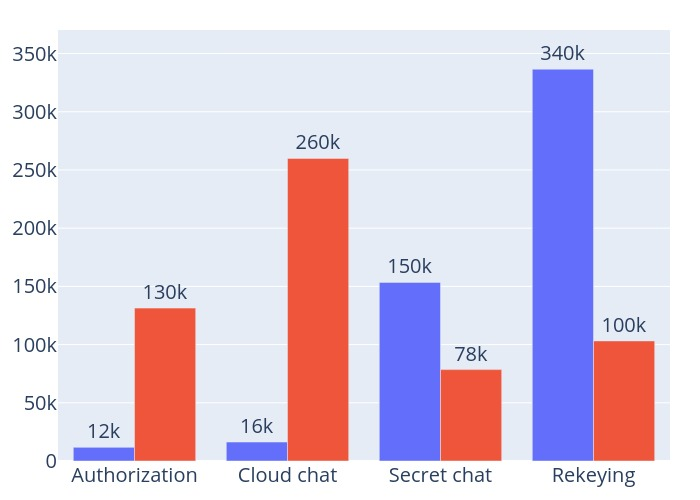
\includegraphics[width=.5\linewidth]{barplot_time}}\hfill
    \subfloat[\Mrss{} (kB)]{\label{b}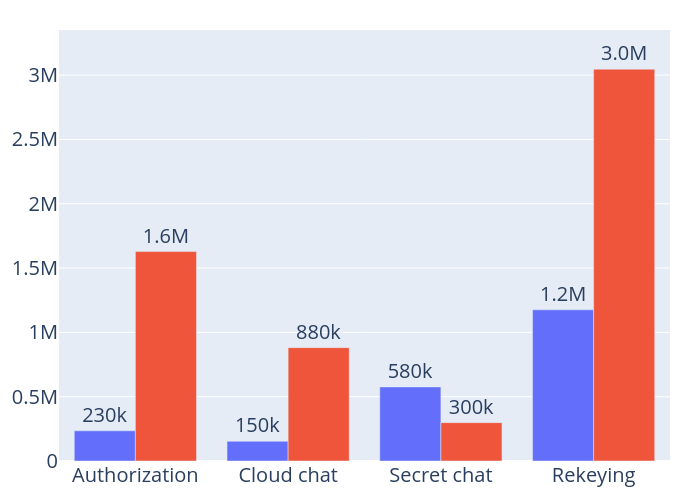
\includegraphics[width=.5\linewidth]{barplot_peak_size}}
    % \subfloat[CPU usage]{\label{c}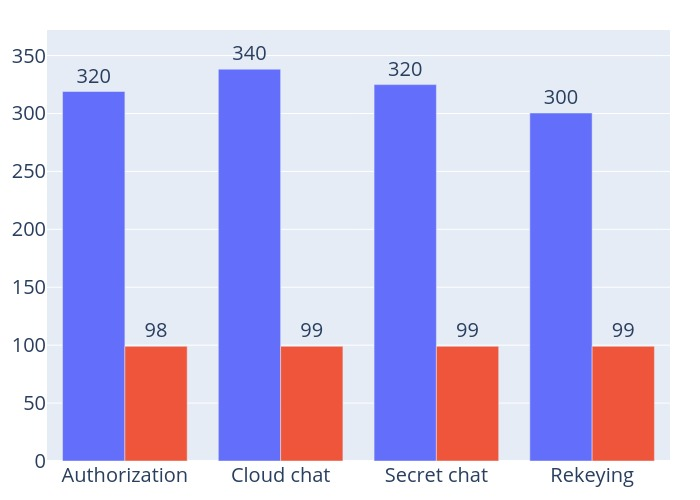
\includegraphics[width=.5\linewidth]{barplot_cpu_time}}
    \caption{In blue Tamarin, in red Proverif.\\\Wct{} and \mrss{} for every protocol and schema.}
    \label{fig:efficiency}
\end{figure}
In this section, we will compare the efficiency of Tamarin's and Proverif's MTProto2.0 formalization. Of course, the measured efficiency is indicative of this implementation only: as a small change can lead to both great performances or non-termination, this is only to be intended as the obtained efficiency of the current version of both implementations.

We consider two different metrics: \textit{\mrss{}} (in kB) and \textit{\wct{}} (in ms).

For the methodology, we followed the same approach of P. Lafourcade and M. Puys \cite{lafourcade:hal-01306395}. Benchmarks were run on an Intel(R) Core(TM) i5-7200U CPU @ 2.50GHz CPU with 16 GB or RAM. To get these three metrics we used the \lstinline{time} command (GNU version) \cite{time_command}. This version of time uses the \lstinline{getrusage} system call, which returns resource usage measures for a process, including our metrics. For each tool and protocol, we executed the proof 40 times. The entire process takes about 12 hours, depending on the hardware. For benchmarks, we used Proverif 2.02pl1 and Tamarin prover 1.6.0. Plots in \cref{fig:efficiency} show the mean value of each execution, while \cref{tab:efficiency} shows many relevant statistics. As we can see, the \mrss{} is usually significantly lower for Tamarin, while the \wct{} differs from protocol to protocol.

\begin{table}[!ht]
    \setlength\arrayrulewidth{1pt}
    \rowcolors{2}{gray!25}{white}
    \makebox[\textwidth][c]{
        \scalebox{0.9}{
            \begin{tabular}{c|cc|cc|c}
                \cline{2-5}
                \multicolumn{1}{l|}{}          & \multicolumn{2}{c|}{\textbf{Peak memory size (kb)}} & \multicolumn{2}{c|}{\textbf{Time (ms)}}                                                                                                                                 \\ \cline{2-6}
                \multicolumn{1}{l|}{}          & Tamarin                                             & Proverif                                & Tamarin   & Proverif  &                                                                                                       \\ \hline
                \multicolumn{1}{c|}{Mean}      & 234707.60                                           & 1628285.70                              & 11726.00  & 131329.50 & \multicolumn{1}{l}{}                                                                                  \\ \cline{1-6}
                \multicolumn{1}{c|}{Deviation} & 4965.62                                             & 149.06                                  & 381.48    & 198.86    & \multicolumn{1}{l}{}                                                                                  \\ \cline{1-6}
                \multicolumn{1}{c|}{Median}    & 234696                                              & 1628286                                 & 11740     & 131270    & \multicolumn{1}{l}{}                                                                                  \\ \cline{1-6}
                \multicolumn{1}{c|}{Min}       & 226000                                              & 1627968                                 & 10880     & 131140    & \multicolumn{1}{l}{}                                                                                  \\ \cline{1-6}
                \multicolumn{1}{c|}{Max}       & 245500                                              & 1628620                                 & 12330     & 131990    & \multicolumn{1}{l}{\parbox[t]{1em}{\multirow{-5}{*}{\rotatebox[origin=c]{90}{\textbf{Auth}}}}}        \\ \hline

                \multicolumn{1}{c|}{Mean}      & 153411.70                                           & 881417.40                               & 16290.50  & 259920.50 & \multicolumn{1}{l}{}                                                                                  \\ \cline{1-6}
                \multicolumn{1}{c|}{Deviation} & 4133.22                                             & 123.44                                  & 238.54    & 469.46    & \multicolumn{1}{l}{}                                                                                  \\ \cline{1-6}
                \multicolumn{1}{c|}{Median}    & 152588                                              & 881388                                  & 16280     & 260015    & \multicolumn{1}{l}{}                                                                                  \\ \cline{1-6}
                \multicolumn{1}{c|}{Min}       & 146384                                              & 881244                                  & 15760     & 259040    & \multicolumn{1}{l}{}                                                                                  \\ \cline{1-6}
                \multicolumn{1}{c|}{Max}       & 163840                                              & 881628                                  & 16960     & 261000    & \multicolumn{1}{l}{\parbox[t]{1em}{\multirow{-5}{*}{\rotatebox[origin=c]{90}{\textbf{Cloud chat}}}}}  \\ \hline

                \multicolumn{1}{c|}{Mean}      & 576006.80                                           & 298242.10                               & 153397.75 & 78498.50  & \multicolumn{1}{l}{}                                                                                  \\ \cline{1-6}
                \multicolumn{1}{c|}{Deviation} & 20908.28                                            & 118.18                                  & 674.64    & 170.40    & \multicolumn{1}{l}{}                                                                                  \\ \cline{1-6}
                \multicolumn{1}{c|}{Median}    & 576940                                              & 298234                                  & 153465    & 78500     & \multicolumn{1}{l}{}                                                                                  \\ \cline{1-6}
                \multicolumn{1}{c|}{Min}       & 529172                                              & 298032                                  & 151200    & 78220     & \multicolumn{1}{l}{}                                                                                  \\ \cline{1-6}
                \multicolumn{1}{c|}{Max}       & 618464                                              & 298488                                  & 154770    & 78940     & \multicolumn{1}{l}{\parbox[t]{1em}{\multirow{-5}{*}{\rotatebox[origin=c]{90}{\textbf{Secret chat}}}}} \\ \hline

                \multicolumn{1}{c|}{Mean}      & 1175407.70                                          & 3046324.80                              & 336571.25 & 103154.25 & \multicolumn{1}{l}{}                                                                                  \\ \cline{1-6}
                \multicolumn{1}{c|}{Deviation} & 14630.59                                            & 206.79                                  & 820.91    & 73.00     & \multicolumn{1}{l}{}                                                                                  \\ \cline{1-6}
                \multicolumn{1}{c|}{Median}    & 1175464                                             & 3046334                                 & 336415    & 103140    & \multicolumn{1}{l}{}                                                                                  \\ \cline{1-6}
                \multicolumn{1}{c|}{Min}       & 1138496                                             & 3045988                                 & 334970    & 103050    & \multicolumn{1}{l}{}                                                                                  \\ \cline{1-6}
                \multicolumn{1}{c|}{Max}       & 1212192                                             & 3046780                                 & 338460    & 103440    & \multicolumn{1}{l}{\parbox[t]{1em}{\multirow{-5}{*}{\rotatebox[origin=c]{90}{\textbf{Rekeying}}}}}    \\
            \end{tabular}
        }
    }
    \caption{Efficiency of the two models for every protocol.}
    \label{tab:efficiency}
\end{table}


\section{Soundness and completeness}
Let us define what soundness and completeness of formal verification tools mean. Definitions are the same given by M. Furer et al. \cite{furer1989completeness}.
\textbf{Soundness} means that any statement that can be proven is valid. A proof system is sound if whenever we can prove something, it is also true. As a formula:

\begin{equation}
    \Gamma \vdash Q \quad \Longrightarrow \quad \Gamma \models Q
\end{equation}

\textbf{Completeness} means that the proof system is powerful enough to prove any valid statement (in some class). In other words, a proof system is complete if whenever something is true, it can be proved to be so. As a formula:

\begin{equation}
    \Gamma \models Q \quad \Longrightarrow \quad \Gamma \vdash Q
\end{equation}

As we can see, soundness is a critical property. Unsound proof systems allow proofs of false statements. In the case of cryptographic protocol verification, this may imply, in the best-case scenario, that the prover yields a proof for a false attack. In the worst case, the tool may miss an attack, which is far more problematic.
Completeness, on the contrary, is a nice-to-have property. Incompleteness means there are some true properties for which there are no proofs in our formal system. \cite{slides_on_sound_complete}.

The foundational papers of Proverif and Tamarin prover respectively assert that:
\begin{itemize}
    \item Proverif is sound, but not complete \cite{ProverifManual};
    \item Tamarin is both sound and complete \cite{TamarinFoundations, TamarinFoundationsExtended, xor_tamarin}.
\end{itemize}



\chapter{Conclusions}
We have shown the two models for cryptographic protocol verification and we have also described the symbolic model in-depth. We have shown how Tamarin prover and Proverif can be used to model a simple protocol. Then, we have presented the MTProto2.0 protocol suite and its formalization using Tamarin prover. We have proved its security in our fully automatic model and we have re-discovered that the protocol is vulnerable to a theoretical \uks{} (UKS) attack. This attack allows a malicious client B, with the help of another client E, to convince client A that she has shared a key with E, while instead she has shared it with B. Finally, we have compared both Tamarin prover and Proverif implementations and found that they have comparable efficiency. However, Tamarin prover excels on the expressiveness, especially considering the powerful built-in theories (such as Diffie-Hellman) available to the user.

Overall, we were able to reproduce the same results obtained with Proverif using Tamarin prover, with some simplifications and restrictions.

%% Fine dei capitoli normali, inizio dei capitoli-appendice (opzionali)
% \appendix

%% Parte conclusiva del documento; tipicamente per riassunto, bibliografia e/o indice analitico.
\backmatter

%% Riassunto (opzionale)
%\summary

%% Bibliografia (praticamente obbligatoria)
\bibliographystyle{plain_\languagename}
\bibliography{thud}

\end{document}